%\documentclass[10pt, twocolumn, nocopyrightspace]{sigplanconf}
\documentclass[letterpaper,twocolumn,10pt]{article}
\usepackage{usenix,epsfig,endnotes}

\pdfpagewidth=8.5in
\pdfpageheight=11in

\usepackage{balance}

% comment out the following line when submitting
%\def \oscardebug{}
%\def \oscardraft{}

% rubber: paper letter

% $Id$
\setlength{\paperheight}{11in}

% natbib package in sigplanconf class file conflicts with cite package
\usepackage{paralist}
\usepackage{times}
\usepackage{graphicx}
\usepackage{rotating}
\usepackage{multirow}
\usepackage{listings}
\lstset{language=C}
\usepackage[hyphens]{url}
\usepackage{comment}
\usepackage{color}
\usepackage{xcolor}
\usepackage{array}
\usepackage{booktabs}
\usepackage[sort]{natbib}
\usepackage{paralist}
\usepackage[hidelinks]{hyperref}
\usepackage{titlesec}
\usepackage{titling}

\renewcommand{\ttdefault}{cmtt}

\begin{document}

%% disable hyperref draft mode for submission

% No copyright block for submission
%\makeatletter
%\let\@copyrightspace\relax5
%\makeatother

%\setlength{\columnsep}{.33in}

% Use the following at camera-ready time to suppress page numbers.
% Comment it out when you first submit the paper for review.
\ifx \oscardraft \undefined
\pagestyle{empty}
\makeatletter
  \let\ps@plain\ps@empty
\makeatother
\fi

%\pagenumbering{arabic}

%\singlespace
%% To make table entries readable
\newcommand\T{\rule{0pt}{2.0ex}}
\newcommand\B{\rule[-0.9ex]{0pt}{0pt}}

% Squeeze space
%\renewcommand{\baselinestretch}{0.99}
%\addtolength{\belowcaptionskip}{-10pt}
%\addtolength{\abovecaptionskip}{-5pt}
%\newcommand{\tabpar}[2]{
%    \begin{center} \begin{tabular}{#1} #2 \end{tabular} \end{center}}

%% \newcommand{\by}[2]{\mbox{#1$\times$#2}}

%% \newcommand{\wunits}[2]{\mbox{#1\,#2}}
%% \newcommand{\um}{\mbox{$\mu$m}}
%% \newcommand{\xum}[1]{\wunits{#1}{\um}}
%% \newcommand{\xnm}[1]{\wunits{#1}{nm}}
%% \newcommand{\sig}[1]{${\tt #1}$}
%% \newcommand{\sigb}[1]{$\overline{{\tt #1}}$}

% Make list indentation tight\
\setdefaultleftmargin{1em}{0em}{}{}{}{}

\ifx \oscardebug \undefined
\newcommand{\fixme}[1]{{}}
\newcommand{\fixmedp}[1]{{}}
\else
\newcommand{\fixme}[1]{{\bf\textcolor{red}{ [ FIXME Ts: #1 ]}}}
\newcommand{\fixmedp}[1]{{\bf\textcolor{red}{ [ FIXME dP: #1 ]}}}
\fi

\ifx \oscardebug \undefined
\newcommand{\note}[1]{{}}
\else
\newcommand{\note}[1]{{\bf\textcolor{blue}{ [ NOTE: #1 ]}}}
\fi

\ifx \oscardraft \undefined
\newcommand{\edit}[1]{{#1}}
\newenvironment{edits}{}{}
\else
\newcommand{\edit}[1]{{\textcolor{blue}{#1}}}
\newenvironment{edits}{\color{blue}}{\color{black}}
\fi

% MW adding. To compile without the red, either:
% (1) comment in the following line:
%\def\noeditingmarks{} % or
% (2) compile with a line like:
%    $ latex '\def\noeditingmarks{} \input osdi08
% Also, might be easier to convert your macros to this format. (I like
% having the comments in another color and also being able to turn them
% all off with one command.)
\begin{comment}
\newcommand{\textred}[1]{\textcolor{red}{#1}}
\ifx\noeditingmarks\undefined
    \newcommand{\pgwrapper}[2]{\textred{#1: #2}}
\else
    \newcommand{\pgwrapper}[2]{}
\fi
\newcommand{\mw}[1]{\pgwrapper{MW}{#1}}
\end{comment}

\newcommand{\intel}{Intel}
\newcommand{\sgx}{SGX}
\newcommand{\sdk}{Intel SDK}
\newcommand{\libos}{library OS}
\newcommand{\libc}{libc}
\newcommand{\sysname}{Graphene-SGX}
\newcommand{\graphene}{Graphene}
\newcommand{\haven}{Haven}
\newcommand{\drawbridge}{Drawbridge}
\newcommand{\scone}{SCONE}
\newcommand{\panoply}{Panoply}

\newcommand{\enclavecallnum}{28}
\newcommand{\palcallnum}{36}
\newcommand{\shieldsyscallnum}{145}

\newcommand{\funcname}[1]{{\tt #1}}
\newcommand{\syscall}[1]{{\tt #1}}

\newcommand{\roughly}{$\sim$}

%%%%%%%%%%%%%%SPACING HACKS%%%%%%%%%%%%%%%

% get the top of the title to exactly 1inch from the top of page
\setlength{\droptitle}{-.55in}     % Eliminate the default vertical space
%%\addtolength{\droptitle}{-4pt}   % Only a guess. Use this for adjustment

% reduce the spacing before \paragraph{} commands: (tweak the number before \@plus)
%% \makeatletter
%% \renewcommand{\paragraph}{%
%%   \@startsection{paragraph}{4}%
%%   {\z@}{0.5ex \@plus 1ex \@minus .2ex}{-1em}%
%%   {\normalfont\normalsize\bfseries}%
%% }
%% \makeatother

%% Eliminate widows and orphans if needed 

% reduce the penalties for page breaks in middle of paragraphs
%% \clubpenalty=10
%% \widowpenalty=10
%% \interlinepenalty=10 %hyphens
%% \brokenpenalty=10    %hyphens

%% \def\topfraction{0.9}
%% \def\bottomfraction{0.9}
%% \def\textfraction{0.1}


% minimize spacing between paragraphs
%% \setlength{\parskip}{0pt}
%% \setlength{\parsep}{0pt}
%% \setlength{\headsep}{0pt}
%\setlength{\topskip}{0pt}
%\setlength{\topmargin}{0pt}
%\setlength{\topsep}{0pt}
%\setlength{\partopsep}{0pt}

%% \addtolength{\voffset}{.3125in}
%% \addtolength{\textheight}{-.0625in}
%% \addtolength{\textwidth}{-.0625in}

%\def\name#1{#1}%
%\def\defname#1#2{\expandafter\def\csname #1\endcsname{\name{#2}}\ignorespaces}%
%\thispagestyle{empty}
%% compress the space between title and authorlist
%\numberofauthors{1}
%\authorinfo{names}{Stony Brook}{emails}
%\author{Anonymous submission to SOSP 2013, please do not distribute. Paper \#162, \pageref*{LastPage} pages total.}
%\author{Anonymous submission to EuroSys 2013, please do not distribute.}

%\titlebanner{Draft, please do not distribute}        % These are ignored unless
%\preprintfooter{Draft, please do not distribute}   % 'preprint' option specified.

\def\longconferencenames{}
\input{../conferences}

%% DP: Note there is a hack in sig-alternate class file to squeeze space under the title for submission.
%\title{Graphene for Shielding: Decentralizing Hardware-Assisted Isolated Execution for Multi-Process Applications}
%\title{Shielding Unmodified Linux Multi-Process Applications with a Multi-Enclave Library OS using Intel SGX}
%\title{Isolating Legacy Applications in Multi-Enclave Environment Using \sysname{} Library OS}
%\title{Shelter the Civilians---Securing Linux COTS Applications with Intel SGX}
\title{Graphene-SGX: A Practical Library OS for Unmodified Applications on SGX}

%\author{Anonymous submission to Security\&Privacy 2017, please do not distribute.}
\author{
{\rm Chia-Che Tsai}\\
Stony Brook University
\and
{\rm Donald E. Porter}\\
University of North Carolina at Chapel Hill \\ and Fortanix
\and
{\rm Mona Vij}\\
Intel Corporation
} % end author

%\vspace{-20pt}}
\date{\vspace{-4ex}} %% compress the space between authorlist and text
%\date{}

\newcommand{\subtitle}[1]{%
  \posttitle{%
    \par\end{center}
    \begin{center}\large#1\end{center}
    \vskip0.5em}%
}

%\subtitle{\bf Draft \today: Please do not distribute}

\maketitle



\titleformat{\section}[block]{
  \fontsize{12}{15}\bfseries}{%
  \thesection}{%
  1em}{%
  }{%
  }%
  
\titlespacing*{\section}
{0pt}{1.5ex plus .1ex}{1ex plus .1ex}

\titleformat{\subsection}[block]{
  \fontsize{12}{14}\bfseries}{%
  \thesubsection}{%
  1em}{%
  }{%
  }%
  
\titlespacing*{\subsection}
{0pt}{1.5ex plus .1ex}{1ex plus .1ex}

\titlespacing*{\paragraph}
{0pt}{.5ex plus .1ex}{1ex plus .1ex}


\setdefaultitem{\normalfont\bfseries\textendash}{}{}{}

\setdefaultleftmargin{1.5em}{3em}{}{}{}{}

\setlength{\abovecaptionskip}{3pt minus 1pt}
\setlength{\belowcaptionskip}{-7pt}

% Use the following at camera-ready time to suppress page numbers.
% Comment it out when you first submit the paper for review.
%\thispagestyle{empty}

\begin{abstract}

  Application partitioning is a technique to move sensitive data or code into
  a protected environment, such as an SGX enclave.
  Partitioning larger existing applications requires subtle reasoning that can be aided with static
  analysis and dynamic, language-level techniques.
  For instance, in-enclave code may include a library that memoizes results in the out-of-enclave heap.
  Using a managed, type-safe language like Java in SGX also brings the benefits of partitioning to a large body of 
  existing code. %, as well as help the developer with language-level analysis tools.
  Unfortunately, running Java partitions in SGX introduces a number of technical
  challenges, many of which arise from resource and system ABI constraints.
  To our knowledge, no prior work has even run a complete Java application in an enclave,
  much less partitioned a Java application to run a piece of application logic in the enclave.
%  That said, no amount of application-level analysis can protect against
%  a compromised OS, without 
  Thus, a number of technical challenges must be addressed to unlock
  the benefit to developers of combining managed languages with hardware such as SGX.


%% \fixmets{Streamlined the argument for combining Java and SGX. Check if this makes sense.}
%% %%There have been significant, but separated %often mutually exclusive,
%% There have been significant, but often mutually exclusive
%% advances in hardware and language-level tools for partitioning applications
%% into multiple security contexts or privilege levels.
%% %Developers who build security-sensitive applications
%% %often face the dilemma of choosing between
%% %managed language features and hardware protections with language restrictions.
%% Developers either 
%% use a hardware solution, such as \intel{} \sgx{},
%% to isolate a piece of consolidated code %small piece of native binary code
%% from an untrusted OS, %but the developer
%% %must reason carefully about potential information flows that could leak data from the enclave, as well as other vulnerabilities in the code.
%% %On the other hand, in
%% or choose to program in a managed type-safe language, such as Java, 
%% %the developer has 
%% which has a wealth of tools and properties for 
%% improving code security and application partitioning.
%% %from type-checking to 
%% %more advanced tools to secure control and information flows.
%% The use of hardware
%% and language-level tools for partitioning are often complementary by concept but incompatible in reality.
%% %mutually exclusive,
%% %due to the limitations in combining the technologies.
%% %This paper observes that these language and hardware security tools 
%% %should complement each other, but are often mutually exclusive.
%% For instance, no language-level analysis %of an application
%% can protect an application against a compromised OS.
%% However, it is fundamentally challenging to
%% factor the protection of \sgx{} into the analysis of a managed type-safe language like \java{}.
%Running a managed language in an enclave is difficult, and language tools
%currently do not factor the hardware capabilities of \sgx{} or similar hardware into their analyses.


%Similarly, the \sgx{} hardware imposes restrictions on loading \java{} classes 
%with \jvm{}s;
%the \java{} language also lacks sensible APIs for using \sgx{} hardware.
%to wrap the semantic of interfaces with the 

%but are not sufficient to defend against a compromised OS or hypervisor.
%but the developer must partition the application 
%and harden the code inside the enclave.
%Managed languages, such as \java{},
%offer a wealth of language-level support for 
%but are not sufficient to defend against a compromised OS or hypervisor.
%The two approaches are often mutually-exclusive:
%we are unaware of any prior work thas has run a \jvm{} inside of an enclave at all,
%For \sgx{} and \java{},
%there is no prior work that has run a \jvm{} inside an enclave,
%much less integrated enclaves into the language's analysis tools.
%\fixmedp{check my claim. Too strong, or justified?}
%\fixmets{Since we are generalizing, we should only claim this is the case for sgx vs. Java. BTW, I prefer showing more certainty when making claims.}


%Application developers can place a library and sensitive data
%in an \intel{} \sgx{} enclave,
%but only if the library is a native binary, generally written in C.
%but must relies on developers to design invulnerable code.

%more advanced tools for detecting information flows.

%These language-level tools can be invaluable in ensuring a correct application partitioning
%and overall application correctness.
%Unfortunately, the most security-sensitive developers must choose between
%hardware and language security tools.


%% Using \intel{} \sgx{} enclaves, applications can
%% protect their most critical components from untrusted system stacks.
%% Language support for \sgx{} enclaves is a missing feature of existing \java{} Virtual Machines.
%% Using a managed language like \java{}
%% provides an opportunity to improve the weakest link of the enclave security---
%% application vulnerabilities that lead to information leakage.
%% \java{} language has effective framework to trace information flows, and provides type safety
%% to prevent memory access vulnerabilities in the enclave.
%% In addition, modularization in \java{} classes allows automatically partitioning
%% an application into enclave components,
%% minimizing the classes included in the enclave's trusted computing base.

This paper presents {\em \sysname{}},
a system that integrates \java{} language tools for partitioning applications
with run-time support for isolated execution in \sgx{} enclaves.
%\fixmedp{Any reason we can't do more than one partition in the enclave?}
%\fixmets{For an application, there is only one partition: the secure-sensitive part. We can create more than one instances in an enclave.}
%and which can execute a portion of the \java{} application in 
%a \java{} utility, runtime framework and API,
%that helps developers design isolated application components,
%and minimizes the attack vectors.
\sysname{} includes both \staticphase{} and \dynamicphase{} components.
The \staticphase{} tool, {\em \statictool{}}, uses code reachability analysis
to determine the minimal required \java{} classes for the isolated execution,
and helps the developer understand the complete partition interface. % between the application partitions.
%\sysname{} helps the developers generate an enclave image
%with minimal required \java{} classes for the protected code, reducing the TCB. %required for isolated execution.
%%\sysname{} includes language-level information flow control at the 
%%enclave border, protecting against unexpected exfiltration of secret
%%data due to application vulnerabilities.
The \dynamicphase{} framework, {\em \dynamicframework{}}, then launches the isolated execution of the enclave image
(a signed JAR archive) in an enclave when the untrusted part calls the interface.
Throughout the execution, \sysname{} enforces end-to-end isolation
on any object instantiated inside the enclave,
and leverages language-level information flow control to determine whether an object contains no sensitive information before the object is released from the enclave.
%to protect against unexpected ex-filtration of secret
%data. % due to application vulnerabilities.
%\fixmebj{How about this?}
%\fixmedp{Is this best-effort?  Only for explicit flows?  The 
%preceding sentence should be crisper}
%identifies information flow at the enclave border,
%preventing enclave secrets
%from being leaked due to any vulnerabilities.
%with minimal classes needed for the isolated computation,
%and narrowest interface for interaction.
%Second, the framework effectively prevents information leakage
%by forbidding any objects tainted by information flow to leave the enclave.
%In \sysname{},
%trusted servers may provision secure objects and classes,
%preserving security policy information. \fixmedp{Don't understand the previous sentence}
%\fixmedp{Do we want to say anything about contributing techniques to get good performance?}
%To secure \java{} applications, 
%With both the \staticphase{} and \dynamicphase{} language support,
\sysname{} also creates language-level abstractions of and extensions \sgx{},
such as attestation and provisioning, simplifying cumbersome aspects of this hardware
for developers.
%extends the security properties (e.g., data confidentiality) and features (e.g., attestation and provisioning)
%of \sgx{}, %hardware protection to cover \java{} classes dynamically loaded by the \jvm{},
%and encapsulates cumbersome aspects of interfacing with the hardware architecture
%keeps the work of bootstrapping and interfacing with 
%from application developers.
%As a proof-of-concept of using advanced language-level tools,
%we use \sysname{} %strengthens hardware protection
%to identify and remove 
%by filtering 
%implicit information flows that would leak secrets from an enclave
 % that leaks secrets
%in our test applications.
%\fixmedp{all of them?  Or just one?}\fixmets{I think this technique applies to all test cases.} % error-prone applications. 
%Finally, the API allows components in enclaves to be seamlessly provisioned with
%secure objects or classes by trusted servers,
%and to preserve their security policy information.
%with security guarantees extended from their sources.
%\sysname{} is evaluated with \jvmname{} on the latest 
%We evaluate \sysname{} % with several case studies 
%on the latest \intel{} Skylake processor.
%Evaluation shows good performance on
%Our overheads are low, 
%adding \fixmedp{xx}\% overhead on an isolated cryptographic library used in SSH client/server,
%and \fixmedp{xx}\% overhead on Hadoop jobs that run a secret, provisioned algorithm.
We demonstrate the usage of \sysname{} with two applications: a SSH server with an isolated cryptographic library to protect its host key,
and a Hadoop framework capable of securely executing jobs using any secret, provisioned algorithm.
%\sysname{} reduces the developer effort required to partition the application code,
%resulting in a smaller 
%and the result of integration is highly generalizable to other managed languages.
%~\fixmebj{Always replace TCB with code footprint size to indicate that we are only talking about size of code - not attack vectors.}
%\fixmets{find a better term for TCB size}
%~\fixmebj{Always replace managed languages with managed type-safe languages.}
%\fixmets{accurately separate managed language and type-safety: managed language causes the challenges, and type-safety improves the security properties; Java happens to be both.
%}
\end{abstract}

\section{Motivation}

Intel SGX introduces a number of essential hardware features that allow an application
to protect itself from the host OS, hypervisor, BIOS, and other software.
With SGX, part or all of an application can run in an {\em enclave}.
Enclave features include confidentiality and integrity protection
for the enclave's virtual address space;
restricting control flow into well-defined entry points for an enclave;
integrity checking memory contents at start time;
and remote attestation.
SGX is particularly appealing in cloud computing, as users 
might not fully trust the cloud provider.
That said, for any sufficiently-sensitive application, using SGX may be prudent,
even within one administrative domain,
as the security track record of commodity operating systems is not without blemish.
Thus, a significant number of users would benefit from running applications on SGX as soon as possible.

Unfortunately, applications do not ``just work'' on SGX.
SGX imposes a number of restrictions on enclave code 
that require application changes
or a layer of indirection. % to work around.
Some of these restrictions are motivated by security, such as disallowing system calls
inside of an enclave, so that system call results can be sanitized by {\em shielding code} in the enclave before use.
%Other restrictions are subtle interactions with unrelated other features, such
%as disallowing the {\tt cpuid} instruction to ensure clear semantics when SGX is combined
%with VT (one mode of VT ensures that using {\tt cpuid} will trap to the hypervisor).
%Intel's SGX SDK includes a limited C library, which is missing a number of features by design.
Our experience with supporting a rich array of applications on SGX, including web servers, language runtimes, and
command-line programs,
%databases (not all are evaluated in this paper), 
is that
a number of software components,
orthogonal to the primary functionality of the application,
rely on faithful emulation of arcane Linux system call semantics, such as \syscall{mmap} and \syscall{futex};
any SGX wrapper library must either reproduce these semantics, or large swaths of code unrelated to security
must be replaced.
Although this paper focuses on SGX, we note that a number of vendors are developing similar, but not identical,
hardware protection mechanisms, including IBM's SecureBlue++~\cite{secureblue++} and AMD SEV~\cite{amd-sme}---each
with different idiosyncrasies.
Thus, the need to adapt applications to use hardware security features
will only increase in the near term.

As a result, there is an increasingly widespread belief that 
adopting SGX necessarily involves significant code changes to applications.
Although Haven~\cite{baumann14haven} showed that a library OS
could run unmodified applications on SGX, this work pre-dated availability of SGX hardware.
Since then, several papers have argued that the library OS approach is impractical for SGX,
both in performance overhead and trusted computing base (TCB) bloat, and that one must instead refactor one's application for SGX.
For instance, a feasibility analysis in the \scone{} paper
concludes that ``On average, the library OS increases the TCB size by $5\times$, the service latency by $4\times$,
and halves the service throughput''~\cite{osdi16scone}.
Shinde et al.~\cite{shinde17panoply} argue that using a library OS, including libc, increases TCB size by two orders of magnitude over
a thin wrapper. % layer, called Panoply.


This paper demonstrates that these concerns are greatly exaggerated:
one can use a library OS
to quickly deploy applications in SGX, gaining immediate security benefits without crippling performance cost or TCB bloat.
We present a port of the \graphene{} library OS~\cite{tsai14graphene} to SGX, called \graphenesgx{},
and show that the performance overheads are comparable to the range of overheads
presented in \scone{};  the authors of Panoply also note that \graphenesgx{}
is actually 5-10\% faster than \panoply{}~\cite{shinde17panoply}.
Arguments about TCB size are more nuanced, and a significant amount of the discrepancies
arise when comparing incidental choices like libc implementation (e.g., musl vs.\ glibc).
\graphene{}, not including libc, adds 53 kLoC to the application's TCB, which is comparable to
\panoply{}'s 20 kLoC or \scone{}'s 97 kLoC. % 
Our position is that the primary reduction to TCB comes from either compiling out
unused library functionality, as in a unikernel~\cite{unikernels} and measured by our prior work~\cite{tsai16apistudy};
or further partitioning an application into multiple enclaves with fewer
OS requirements.
%, such as just
%terminating a TLS connection in the enclave.
When one normalizes for functionality required by the code in the enclave, the design choice between a library OS or a smaller shim does not have
a significant impact on TCB size.

To be clear, SGX-specific coding has benefits, but we must not let the perfect be the enemy of the good.
For example, privilege separating a complex application into multiple enclaves may be a good idea
for security~\cite{flicker,Provos:2003:PPE:1251353.1251369,shinde17panoply}, and replacing particularly expensive operations can improve performance on SGX.
%Our experience with supporting a rich array of applications on SGX, including web servers, language runtimes, and
%databases (not all are evaluated in this paper), is that
%a number of software components orthogonal to the primary functionality of the application
%rely on faithful emulation of arcane semantics of Linux system calls, such as {\tt mmap} and {\tt futex}.
The goal of \graphene{} is to bring up rich applications on SGX quickly, and then let developers
optimize code or reduce the TCB as needed.

\graphenesgx{} runs unmodified Linux binaries on SGX; to this end,
this paper also contributes a number of usability enhancements,
%\fixme{check this}
including integrity support for dynamically-loaded libraries,
%remote attestation,
enclave-level forking, and secure inter-process communication (IPC).
Users need only configure features and cryptographically sign the configuration.
\graphenesgx{} is also useful as a tool to accelerate SGX research.
%\graphenesgx{} has been open-sourced since June 2016\footnote{Available at https://github.com/oscarlab/graphene}.
Although our focus is unmodified applications, \graphenesgx{} can also run smaller pieces of
code in an enclave, as in a partitioned application.
Several papers already compared against or extended 
\graphenesgx{}~\cite{shinde17panoply, orenbach17eleos, kim2017enhancing}
%\fixmedp{I think there are more - Chia-Che please check recent google scholar activity}\fixme{these are all I can find; others are all just citing Graphene as related work}, 
and we are aware of ongoing projects using \graphenesgx{}.
%One published paper has already benchmarked against Graphene-SGX~\cite{shinde17panoply},
%and we are aware of a number of concurrent submissions to other conferences that
%use Graphene as either a building block or comparison point for software that uses SGX.
%In a short time, Graphene-SGX has already had significant use outside of this group,
%Has already been benchmarked in published papers by other groups.
%We are aware of several concurrent submissions to other conferences that are
%buiding extensions to Graphene


\begin{comment}
The contributions of this paper are:
\begin{compactitem}

\item A framework, called \graphenesgx{}, to isolate unmodified, Linux  applications in enclaves.
%providing sufficient Linux compatibility and complete isolation from the untrusted OS.
%A platform (referred to as ``\graphenesgx{}'' for the rest of paper) as basic blocks of porting application binaries under SGX isolation,
%and reusing most of the legacy code and supporting libraries to minimize the development effort.
%\graphenesgx{} extends the \graphene{} \libos{} to support Linux features upon a narrow interface to untrusted hosts.

\item Several usability enhancements for SGX, including
  dynamic loading, \syscall{fork}, and IPC.

%  \graphenesgx{} narrows the enclave interfaces until the security of each enclave entries can be studied and reasoned about.
%The primary challenges include enforcing attestable application integrity and isolating multi-process abstractions (e.g., fork, IPC, namespaces).
%\fixmedp{huh?}

%\graphenesgx{} shields \shieldsyscallnum{} Linux system calls for applications,
%by authenticating the inputed resource (e.g., files) to the host interface.
%Especially, \graphenesgx{} shields multi-process system calls, including \fork{}, \exec{}, signaling, namespaces, and system V IPC, 
%for applications that span across multiple enclaves.

\item A thorough evaluation of the performance of unmodified applications on \graphenesgx{}, indicating
  that the costs of a feature-rich library OS on SGX are in-band with purportedly lighter-weight solutions
  that require application changes.  For example, lighttpd throughput and latency on \graphenesgx{} are comparable
  to a Linux process.
  Overheads are generally under $2\times$ (cf.\ \scone{} overheads up to $1.6\times$ on comparable workloads).
  In a few cases, \graphenesgx{} overheads are higher, but these are internal to the library OS
  or fundamental to enclave limitations, %initialization costs or memory limitations,
  not because the application is unmodified.
%  \fixmedp{Any more specific nuggets here?}
  

  %Based on the experience of deploying \graphenesgx{} in systems, we identify several challenges in running COTS applications in enclaves, including performance factors and security issues. \fixmedp{vague}

%\graphenesgx{} realizes a deployment model (as shown in Figure~\ref{fig:deploy-model}) that transits Linux COTS applications to \sgx{},
%without the individual effort of porting the applications.
%\graphenesgx{} divides up the three goals of \sgx{}: isolating execution, attesting code integrity and authenticating trusted enclaves---\graphenesgx{} centralizes the effort of bootstrapping the isolation, and assists developers to accomplish the other two goals.
\end{compactitem}
\end{comment}



%I think the story here is that fears of the costs of library OSes are greatly exaggerated, and the performance is fine + it is easy to use.  Although SGX has a lot of limits, it doesn't have to be hard to bring up code on SGX (or other upcoming secure HW platforms) quickly.
%* Yes, you can do better with custom code in swift or whatever, but a lot of people benefit from thunking code down and having it "just work" with protection
%To this end, we also contribute usability enhancements, like dynamic linking, remote attestation, ipc, fork, etc.
%We contribute a measurement of a relatively mature SGX libos on real hardware.
%Shit works, lots of people are using Graphene.

%This chapter describes the formal definition of the \graphene{} host ABI.

\section{Basic Definitions}

The \graphene{} host ABI defines a set of {\em functions}, similar to the API of UNIX or POSIX.
The functions are directly called by the library OS, along with the arguments given either in the registers or on the stack.
A host-specific \graphene{} loader is responsible for resolving the linking, from the library OS to the host ABI.
\papersection{Challenges for Partitioning with Enclaves}
\label{sec:background}
In this section, we will give a brief overview of \sgx{}, and discuss 
the key challenges developers face when trying to manually partition applications using a technology such as \sgx{}.
%discuss the programming models and threats to security of \sgx{} enclaves.

\papersubsection{Background on \intel{} \sgx{} Enclaves}

\intel{} \sgx{} ({\it Software Guard Extension})
is a set of new x86/x64 instructions
introduced in the \intel{} Skylake processor family.
Using \sgx{}, an 
application can designate part of its virtual memory as an {\em enclave}.
The CPU guarantees that the contents of the enclave never leave the CPU package unencrypted.
The CPU also measures the integrity of a binary loaded into the enclave, and offers remote attestation,
similar to a TPM\fixmedp{cite}.

%%% create a protected memory region, called an {\em enclave}, inside it's virtual memory,
%%% where it can load its security sensitive data with hardware-enforced isolation from the untrusted OS. 
%%% The processor with \sgx{}
%%% guarantees that any data loaded in enclave
%%% stays encrypted in the DRAM, by using a secret key deterministically derived from the application's cryptographic measurement and the CPU secret. 

\sgx{} is an appealing tool for protecting small amounts of highly-sensitive data or code, because it can defend 
against a malicious or compromsed OS, hypervisor, or even hardware peripheral.
For instance, \fixmedp{Foo} et al.~\fixmedp{cite that \sgx{} workshop paper} show how \sgx{} can be used
to build a trusted path from a video chat application to a GPU and network card, which maintains confidentiality and integrity of the
video stream, even if the OS is compromised.
Simlarly, because DRAM contents are encrypted, \sgx{} can resist cold-boot attacks~\cite{halderman09coldboot} or 
malicious peripheral devices~\cite{hudson15thunderstrike}.


%%% \sgx{} also proves the integrity of loaded binaries to remote trusted entities
%%% using mutual attestation based on a symmetric key generated from the measurements of communicating entities.
%%% \sgx{} usage model mostly involve the launched enclave mutually attesting the trusted host
%%% to obtain provisioning of security-sensitive information
%%% through a trusted channel. Such an execution model leverages resources such as CPU and DRAM from vulnerable untrusted \sgx{}-enabled hosts owned by cloud providers
%%% by extending the trust from
%%% the hosts owned and trusted by the clients or service providers.
%%% For instance, \sgx{} can isolate the decoder engine in an enclave
%%% after authenticating the customers to enforce Digital Right Management (DRM) even if the digital data is hosted on an untrusted cloud server.

%Use cases of \sgx{} mostly involve the launched enclave
%retrieving a cryptographically signed attestation from the processor,
%to exchange security critical information with remote servers through secured channels.
%The effect is equivalent to expanding the trusted space from remote servers
%to the local end, to harness local resources such as CPU and DRAM.

%One must note that \sgx{} only promises the integrity of application binaries
%initially loaded in enclaves.
%The gap between integrity of binaries and complete security has to be filled
%by ones who develop and approve the applications.
%More specifically, the clients are responsible of
%testing whether the applications contain any vulnerabilities
%that lead to information leak.
%To minimize the risk of leaving any flaws in the applications unintentionally,
%developers often tend to cut down the trusted computing base (TCB)
%of the applications. With smaller TCB, clients who launched the enclaves
%can more easily reason about the thoroughness of securing the execution.

%%% The key strength of \sgx{} enclaves over other software-based isolation framework such as
%%% {\em Flicker}, {\em Inktag} or {\em Virtual Ghost} is
%%% the ability to defend against attacks at the hardware level.
%%% These software-based solution often
%%% rely on a hypervisor below the OS to isolate the applications.
%%% If the hardware is attacked,
%%% the attackers may still bypass the software checkpoints,
%%% or directly steal confidential information from the DRAM.
%%% For \sgx{}, the only hardware included in the TCB is the CPU package,
%%% and in practice CPUs are believed to be hard to attack.
%%% Using techniques like cold-boot attacks~\cite{halderman09coldboot}
%%% to peek into DRAM content,
%%% or intruding the boot process using corrupted peripheral devices like Thuderstrike~\cite{hudson15thunderstrike}
%%% will affect any software-based isolation, but not \sgx{} enclaves.

\paragraph{Non-Partitioned Applications.}
One approach to using \sgx{} is to run an entire application in the enclave.
This is exemplified by Haven~\cite{baumann14haven}, which runs a \win{} application and all supporting libraries
on top of a {\em library OS}.  This approach is illustrated on the left side of Figure~\ref{fig:libosvssdk}.
The library OS approach does not require any application changes, but bloats the TCB \fixmedp{Rough number of how big Haven is}.
By pulling millions of lines of extraneous code into an enclave, there is a significantly increased risk 
of vulnerabilities that disclose
sensitive data, such as Heartbleed~\fixmedp{cite}.
The library OS approach is useful in its simplicity of deployment and can provide practical benefits, 
such as protecting an application from an untrusted cloud hypervisor.

\begin{figure}[t!]
\centering
\includegraphics[width=\linewidth]{figures/libosvssdk.pdf}
\footnotesize
\vspace{-0.2in}
\caption{
Comparison between the libOS-based model (e.g., Haven)
and the partitioned model for programing applications in enclaves.
Green (light) boxes are trusted components and red (dark) boxes are untrusted.
The libOS-based model yields a larger TCB in the enclave,
while the partitioned model requires developers to be responsible for determining the untrusted interface at the enclave boundary.
}
\label{fig:libosvssdk}
\end{figure}


This paper focuses on a second usage model for enclaves, where the application is partitioned into
untrusted and one or more trusted components (right side of Figure~\ref{fig:libosvssdk}).
Sensitive data and computation are placed inside of enclaves.  This approach requires the developer to
identify sensitive code and data; design and harden an interface between trusted and untrusted components; 
modify the application source; and reason about potential information flows at the enclave boundary.
This effort can be non-trivial and subtle, but for application developers motivated by interests such as 
regulatory compliance or competitive advantage in business, the additional effort can yield a much smaller trusted computing
base (TCB), and thus a reduced attack surface.
A key goal of \sysname{} is to minimize the developer's effort to partition an application---both in lines of 
code changed, and in leveraging language analysis to reason about narrow points in the application's data and control flow.


%To achieve smaller TCB, the software development kit of \sgx{}
%intends to encourage developers to partition the applications and
%keep only security sensitive components in the enclaves.
%Such an intention is exactly contradicted by the trust model of \haven{},
%which must trust the loaded application as a whole.
%Except for the cases in which the whole applications must be secured,
%\haven{} actually downgrades the trustworthiness of enclaves.
%Figure~\ref{fig:libosvssdk} shows the comparison of the two models.

%%% In prior works using \sgx{} enclaves to secure applications,
%%% developers choose between two different programing models: the {\em library-OS-based} and the {\em partitioned} model (as shown in Figure~\ref{fig:libosvssdk}).
%%% In the libOS-based model, developers run the whole standalone,
%%% legacy application inside the enclave, using library OS such as {\em Haven} or {\em Graphene libOS} to facilitate the rich OS features.
%%% The main benefit of using library OS is that developers only have to employ minimal efforts to port any existing application.
%%% Even when designing new applications, developers bear no responsibility
%%% of identifying and reasoning about
%%% the security sensitive part of the application.

%%% However, when using libOS-based model, a sophisticated legacy application
%%% will yield huge trusted computing base (TCB) in the enclave,
%%% aggravating the risk of leaking information through vulnerabilities inside the enclave.
%%% Known bugs such as {\em the heart-bleeding bug} has shown that
%%% running security sensitive code like an encryption engine, and management code such as heart-beating service in the same address space
%%% can cause vulnerabilities that compromise the security by leaking the encryption key.
%%% As a result, using a partitioned model, developers can isolate only the most security sensitive components in an enclave,
%%% and leave the remaining code outside to minimize the TCB.

%%% Developers have to define the {\em untrusted interface} 
%%% to allow parts of a partitioned applications to interact.
%%% The untrusted interface is used either by the the untrusted components
%%% to trigger execution of the isolated components,
%%% or by isolated components to use untrusted rich OS features, such as networking for provisioning and sending the execution output to the remote hosts.
%%% Unlike the libOS approach that has a fixed untrusted interface (for different applications) at their interaction boundary with the OS,
%%% the width of untrusted interface for a partitioned application is up to developers' design.
%%% The \intel{} SDK for \sgx{} supports a set of syntaxes to specify the type and direction of flow for parameters of the untrusted interface, and enforces primitive
%%% type-checking of incoming values on transition to enclave.

%%% The trade-off between the libOS-based and partition model is based 
%%% on ease of development, the width of untrusted interface,
%%% and size of TCB.
%%% The benefit of the libOS-based model is that developers can save the effort
%%% of determining what to execute in the enclave,
%%% and whether the execution is safe,
%%% because the whole application is wrapped in the enclave.
%%% However, the risk of having vulnerabilities in the applications
%%% is not reduced, but in fact amplified due to the addition of
%%% the library OS (e.g., the Haven binary yields around a few hundred MBs) to TCB.
%%% On the other hand, if the developers are willing to spend effort on carefully identifying the untrusted interface and re-designing their application around this interface, the partitioned model can improve security guarantees by minimizing the attack vectors.

%%% The goal of \sysname{} is to provide the benefits of both models.
%%% \sysname{} support a partitioned model
%%% for developers to isolate security-sensitive part of a \java{} application in enclave,
%%% and provide a language-based tool to automatically partition
%%% the minimal supporting classes to generate the enclave image.
%%% Even in the case where the isolated component need to frequently interact with the untrusted component or the OS,
%%% the language protection technique of information flow tracking
%%% guarantees that the secrets in the enclave are never leaked
%%% without the developers explicit consent. 

\paragraph{Side Channels and Denial-of-Service.}
In the current \sgx{} design, side channels are a signficant concern for either the library OS or partitioned model, and are out of the scope of this paper.
A controlled channel attack~\fixmedp{cite} can single step enclave execution by inducing page faults
in the enclave.  \sysname{} does not specifically defend against side channel attacks,
and we expect that any solution to this problem involves redesigning the division of labor in virtual
memory management for enclaves.

Similarly, there is no guarantee that a compromised application will ever enter
an enclave.  Denial-of-service attacks are out of scope for this paper.


\papersubsection{Challenges for Application Partitioning on \sgx{}}

\sgx{} provides useful building blocks for secure applications, but does not
absolve the programmer of any responsibility for reasoning about end-to-end security.
Bugs in the application or supporting libraries can still disclose sensitive data from an enclave,
and porting code into \sgx{} can be subtle.
This subsection outlines several pitfalls in partitioning an application for \sgx{}.

%%% \sgx{} enclaves provide strong isolation guarantee for applications,
%%% against the malicious or vulnerable application components, system stack,
%%% and hardware (except the CPU itself).
%%% However, the security guarantees of the \sgx{} enclave is dependent on whether the developers design perfect applications without exploitable vulnerabilities that may compromise the application's security.
%%% As the application developers are not perfect,
%%% even applications or components isolated in enclave can face threats to their security.
%%% As follows, we discuss a few potential threats
%%% to the enclave security,
%%% even under the assumption that the \sgx{} hardware is implemented as completely secure --- which can be another threat otherwise. 

%\fixmedp{I roughly want the rest of this section to have a problem, explanation, solution structure, with the overall theme being that this is subtle and we really need some analysis tools to get this right}

\paragraph{Writes outside of the enclave.}
\sgx{} allows code inside the enclave to read and write data structures 
outside of the enclave.  Thus, it is easy for a developer to inadvertently write
code that discloses a secret, say by using a library that memoizes intermediate results to the untrusted heap.
A fundamental requirement is that developers must be able to reason about (or assert)
what code can and can't access data {\em outside} of the enclave.
\fixmedp{Can we say anything about whether such tools exist before Civet?}

%\fixmedp{Do I recall correctly that you can easily write to data outside of the enclave?  If so, this seems like something easy to get wrong, especially 
%if a library memoizes intermediate results.  The developer needs to be able to tell 
%Unless I am full of shit, can we paragraph-ize this fixme?

\paragraph{Application vulnerabilities.} 
The major source of threats to enclave security is any internal vulnerabilities in the isolated components,
such as buffer overflows and other memory corruption attacks.
Moreover, although \sgx{} code integrity guarantees make enclaves resistant to code injection,
an attacker may still manipulate control flow using code-reuse attacks~\cite{code-reuse-attacks}.
Moreover, recent research ~\cite{hudata} show that even with perfect control flow integrity,
attackers can still manipulate the execution to leak the secrets through information flow.

Fundamentally, this argues for some combination of static analysis
and runtime monitoring of 
enclave code.  This is greatly simplified when the enclave code is written in higher-level languages
with properties 
%amenable to analysis.
%with type safety, memory safety, and other 
%that provide important 
%safety properties,
such as type safety or memory safety. %, thereby reducing the likelihood of these vulnerabilities.
Ideally, one would formally verify security properties of enclave code~\cite{moat}; this verification is significantly aided by using 
higher-level languages amenable to formal reasoning.
%Verification is significantly harder
%with C or x86 assembly.

%% \paragraph{Applications are not perfect} 
%% The \sgx{} hardware cannot prevent applications from copying secrets out of the enclave without limiting functionality.
%% The trusted isolated components can copy any sensitive data from the enclave to the unencrypted memory, and potentially leak the enclave secrets.
%% The primary risk in the isolated components
%% is often memory corruption vulnerabilities, such as buffer overflow,
%% %Because in enclave applications can access any part of out-of-enclave memory unrestrictedly,
%% prevalent in applications that are not implemented in type-safe languages.

%% The best known technique to prevent vulnerabilities is to model the applications and verify them using {\em formal verification}.
%% While Sinha et.al.,~\cite{moat} use formal verification to prove confidentiality of enclave programs, it is impractical to accurately model complex sophisticated applications.
%% As a result, in addition to formal verification, maintaining smallest TCB
%% in the isolated components is the most practical approach 
%% to ensure enclave security,
%% and is the main reason to choose partitioned programming model over
%% libOS-based model.


\begin{figure}[t!]
\centering
\includegraphics[width=\linewidth]{figures/partition.pdf}
\footnotesize
\vspace{-0.3in}
\caption{
Partitioning --- either manually or by automated tool ---
often causes wider boundary of partition than the actual security sensitivity boundary
due to (a) design granularity : {\tt secHelper} contains a {\tt send()} method that is not partitioned from the rest of the class by design.
The reasons of having the gap vary, for instance, 
that is less security sensitive, but due to the granularity it is not partitioned from the rest of the class or (b) better performance :  the less security sensitive {\tt logger} class is kept in the privileged level to service frequent method calls.
}
\label{fig:partition}
\end{figure}

%However, even if developers partition the applications and run only
%security sensitive components in the enclave,
%the developers may still leave some code irrelevant to
%enclave secrets inside the enclave.
%The reasons of having more-than-minimal TCB in enclaves
%are often that developers have to partition code in the granularity of source files or functions,
%or developers have to import more code to limit the width of interface and
%the frequency of interaction with the untrusted code.

\paragraph{Identifying ``pinch points''.}
Reasoning about where in a program to draw the line between 
trusted and untrusted code is subtle.
On one hand, the developer has an incentive to minimize the size of the 
API between the enclave and untrusted code, as well as an incentive to
minimize the total code in the enclave.  These goals can sometimes be at odds.
Each entry and exit to an enclave has a cost roughly comparable to a
process context switch\fixmedp{right?}; an easy way to reduce enclave entries and exits is to simply 
pull more code into the enclave, which increases the size of the TCB.

\fixmedp{I'm not sure how to explain Figure~\ref{fig:partition}, but it needs an explanation.}

Fundamentally, the art of paritioning an application is to find a ``pinch point'' or
``narrow waist'' in the application, where there is a natural point to insert an API and 
security checks.  This is indeed as much art as science, often done manually by experts\fixmedp{any more supporting evidence or cites?}.
It is unlikely that the average developer will successfully navigate this design process without analysis tools, such as \fixmedp{examples?},
to help identify these natural division points.


%% Experts can use a manual partitioning technique to achieve smallest TCB for the isolated components compared to automated tools.
%% However, the manual partitioning costs a lot of effort,
%% and rare expertise, lack of which can cause larger TCB.

%% Neither manual nor automated partitioning is perfect:
%% the resulted boundary of partitioning often has a gap from the actual boundary of security sensitivity (as shown in figure~\ref{fig:partition}),
%% leaving more code in the privileged level
%% than what's actually needed.
%% Having the gap between the ideal and resulted boundary
%% is mostly inevitable, due to multiple reasons.
%% One common reason is the granularity of partitioning,
%% which can vary from a binary file, a component, a source file,
%% a class, a method (a function) to a line of code.
%% Another reason is that a component or a method may be too frequently called
%% by the security sensitive code,
%% laying the boundary between the component or method from the security sensitive side may bring too much overhead or risk,
%% because the execution crosses the boundary too often.
%% Therefore, developers often will balance among the effort of partitioning,
%% risk or cost of communicating between different partitions,
%% and minimizing the TCB in the security sensitive parts.

\fixmedp{Maybe move the commented paragraph below down into the design section?  I'd like to downplay the plugs for our work here, and instead fulfill these promises later}
%% \sysname{} automates partitioning of applications,
%% based on the boundary at the classes which the developers marked
%% as the interfaces of the enclave.
%% Only the classes that are depended by the marked classes
%% will be included in the enclaves,
%% to minimize the TCB.
%% Although not all classes pulled into the enclaves
%% are necessarily security sensitive,
%% the enclaves are protected from the potential vulnerabilities in those classes,
%% by the security guarantees of \java{} language,
%% and the information flow tracking in \sysname{}.

%Another threat to \sgx{} is the vulnerability of the 
%security sensitive code running in the Enclave. The 
%main guarantee of \sgx{} to isolate the secure data 
%from other components and privileged OS is undermined 
%if the Enclave code can be tricked to leak the 
%security sensitive data to the attacker. Executing 
%buggy code in \sgx{} enclave can inadvertently leak 
%information if the attacker can exploit memory-safety 
%vulnerabilities like buffer overflow and dangling 
%pointers.  

% Cumbersome and approximation to partition code
%The developers have to manually partition their code 
%into security sensitive and insensitive part. If this 
%partitioning is done by a novice developer, some of 
%the security insensitive parts of the application can 
%end up in the security sensitive part, increasing the 
%Trusted Computing Base(TCB). Moreover, the 
%partitioning of code is not straightforward, which 
%can also contribute to a less stricter TCB. The bigger the TCB, the more %vulnerable is the Enclave code to attacks.

% Buggy Code leads to inadvertant information leakage


% \sgx{} code only Integrity protected not confidential
%Moreover, \sgx{} only protects the integrity of the enclave code. The security critical part of the application is stored in plaintext while the secret data is provisioned securely after attestation. However, \sgx{} does not protect the confidentiality of enclave application code which may be executing a secret algorithm. \fixmebj{Talk more about the problem motivating security tag preservation.}
%\sgx{} can natively guarantee either code integrity or
%code confidentiality (as part of the enclave data), but not both.
%If application code is included in the enclave measurement and
%verified by the hardware,
%the code must stay in plaintext as part of the enclave image.
%If any code is stored or provisioned in encrypted forms,
%the application or infrastructure in enclave must dynamically load
%the code after decryption.
%Supporting dynamic loading makes enclaves open to code injection
%if the applications have exploitable vulnerabilities.

\paragraph{Code Integrity {\em and} Confidentiality.} 
The hardware-level \sgx{} code integrity mechanism is based on a cryptographic
signature of a static binary in plaintext.
If any application dynamically loads any code after the enclave's initial measurement,
the initial application must be trusted to attest the loaded code.
The subtle tension is that there is no way to protect the confidentiality of
a secret algorithm, except by dynamically loading an encrypted binary.
Dynamically loading code increases the risk of code injection attacks and other control flow compromises.

Any application partitioning solution that protects sensitive algorithms
must have a robust dynamic loader that can measure encrypted libraries or classes.
\sysname{} includes a loader that can measure encrypted class files,
provisioned from a trusted host.

%% \sgx{} enclaves require code integrity in the isolated applications.
%% If the code integrity is not maintained, adversaries can corrupt the enclave code to
%% force the applications to leak the information provisioned from the remote,
%% trusted hosts.
%% \sgx{} hardware only guarantees
%% the integrity of the code initially loaded into the enclaves.
%% However, if an application choose to dynamically
%% load any code after the enclave starts,
%% the application is responsible for the integrity of the code loaded.
%% The fact that dynamic loading of applications, libraries or components
%% is a feature that can potentially make enclaves vulnerable and open to code injection,
%% raises concerns against supporting managed languages in the enclaves.

%% On the other hand, code confidentiality can be a desirable feature,
%% for application developers who prefer keeping the secret sauce of their algorithms concealed.
%% To enable the feature of code confidentiality in enclaves, the protected code must be dynamically loaded into the enclave,
%% because the \sgx{} hardware only accept
%% the initial loaded code to be in plaintext.
%% \sysname{} provides both code integrity and confidentiality by verifying
%% every classes dynamically loaded into the enclaves,
%% and allows loading classes provisioned from trusted hosts.


%% In general \sgx{} enclaves are prone to having side channels, such as timing channels. Because \sgx{} relies on the untrusted OS for paging,
%% an enclave will always leak page fault addresses, except the lower 12 bits (offsets in pages).
%% Such a leakage gives the untrusted OS to amplify the side channels,
%% by forcing page faults on every instruction or memory access.
%% This so-called {\em Controlled Channel Attack} is common to all applications who use \sgx{} protection, regardless of the programming models.
%% \sysname{} does not specifically defend against side channel attacks.

%% \paragraph{Denial-Of-Service Attacks}
%% \sgx{} is not designed to be safe against denial-of-service attacks.
%% Because the untrusted OS still controls the host resources,
%% there are countless ways to prevent an enclave from making progress.
%% For example, the OS can simply starve the enclaves by
%% never scheduling CPU, memory or other resources to the enclaves.
%% \sysname{} does not specifically defend against denial-of-service attacks.

\paragraph{Discussion.}  This
section has outlined several pitfalls for developers of partitioned applications.
These common pitfalls render the hardware protections of \sgx{} useless.
Language-level analysis can automate error-prone reasoning in the best case, or, in the worst case, 
can at least offer invaluable guidance to the developer.  For \sgx{}-style
hardware to be useful to a wide array of developers, developers need language-level
tools that can also factor in hardware-level protection mechanisms.



%- Motivate the problem.
%- List all attack vectors
%- How can JAVA help?




















































































%\section{Minimizing the TCB with the Non-Partitioned Model}

%\subsection{Reducing the TCB in \libos{}}
%\subsection{Partitioning the TCB in Multi-Process Applications}



\papersection{Overview of the \sysname{} System}
\label{sec:overview}

This section provides an overview of \sysname{},
a system that assists developers in partitioning \java{} applications,
by combining \sgx{} hardware protection and \java{} analysis tools.
%with hardened security from both \sgx{}'s security guarantees and 
%\java{}'s safety features.
%% dep
%We will also discuss the threat model assumed in the design of \sysname{}.

\begin{comment}

%\begin{figure}[t!]
%	\centering
%	\includegraphics[width=\linewidth]{figures/alternatives.pdf}
%	\footnotesize
%	\caption{Alternative approaches to access \sgx{} hardware protection from \java{} applications.
%		The {\em libOS-based} approach runs the whole \java{} applications in the enclaves. 
%		The {\em JNI-based} approach uses JNI to run the security sensitive operations inside the enclaves.
%		The {\em \jvm{}-based} approach requires the \jvm{} to provide APIs to support common use cases of the enclaves.
%		Green (light) boxes are trusted components and red (dark) boxes are untrusted.
%	}
%	\label{fig:alternatives}
%\end{figure}

There are multiple approaches to access \sgx{} hardware from \java{} applications as illustrated in Figure~\ref{fig:alternatives}. Firstly, the whole \java{} application can run with the \jvm{} inside the enclaves,
using a \sgx{} like Haven~\cite{baumann14haven}({\em libOS-based}).
Secondly, the untrusted components of \java{} application
can run with the \jvm{} outside the enclaves, and a JNI wrapper can communicate
with the trusted component written in native language running inside the enclave like ~\cite{vc3}({\em JNI-based}). 
However,the JNI-based approach requires developers to have the knowledge of
enclave implementation, and loses the language protection of \java{} inside the enclaves.
A more plausible approach is to provide enclave-backed APIs
from the \jvm{},
to support common use cases ({\em \jvm{}-based})), such as a secure key-value store~\cite{vc3}.
Although the \jvm{}-based approach can save the application developers' effort
of implementing isolated components,
the use cases is limited to the pre-defined operations provided by the \jvm{} or the companion frameworks.
Because the backend implementation (isolated components and untrusted interfaces) in the \jvm{}-based approach is the same as the JNI-based approach,
the same language restriction also applies here. 

\end{comment}

\papersubsection{Design and Features}

\sysname{} consists of a \staticphase{} tool (\statictool{}) and a \dynamicphase{} framework (\dynamicframework{}):
%to help 
%developers to partition \java{} applications.

\paragraph{Partitioning \java{} applications into enclaves (\statictool{})}
To cleanly partition \java{} applications into
 trusted and untrusted components,
 \sysname{} provides a \staticphase{} tool called \statictool{}
%\fixmedp{I recommend naming each component: ``Shredder'' vs. ``the Civet design-time tool''} 
 to automate partitioning.
 In a \sysname{} partition, there are three types of classes.
 First, the developer will identify trusted classes that must execute
 exclusively in the enclave, called an entry class.
 \statictool{}  will identify functions and supporting classes that are reachable
 from the enclave.
 The developer will then decide which additional classes can be instantiated
 only in the enclave, which can be instantiated inside and outside of the enclave, and
 which can only be created outside of the enclave---essentially forming a border
 for the partition.
%The developer manually identifies trusted classes that should be placed in the enclave,
%but will still interact with untrusted components.
%These classes are called entry classes for the enclave.
%Based on the list of entry classes, 
%Shredder selects all supporting classes required by the entry classes,
%the minimal supporting classes that the entry classes have dependency against,
 \statictool{} creates a static image of the in-enclave java classes, packaged as a signed JAR file.
 
 \sysname{} partitions at class granularity, but enforces isolation at  object-level.
 In other words, some classes can execute both in and out of the enclave,
 such as a generic container class or the String class; in these cases,
 the runtime isolation granularity is  object-level (whether it is placed
 in the enclave heap or the untrusted heap).
 \sysname{} does not currently remove unused functions from in-enclave classes,
 although this enhancement could be adopted in future work.
  

%The developer can request for other non-sensitive classes or packages to also be included in the enclave JAR file.
%\fixmedp{Can the developer override this if she wants to exclude some packages, or replicate some packages, rather than share them?  What if she wants instances of the same class in and out of the enclave?}


% \fixmebj{Talk about class level partition granularity and object level isolation granularity.}
%\sysname{} asks the developers to identifies the trusted classes that must be isolated in the enclave,
%but interact with the untrusted components.

For most cases, \sysname{} only requires the developers
to identify the entry classes, and, as desired, to annotate declassifiers for information flow tracking (\S\ref{sec:concept:accessing}).
Our goal is to minimize developer effort required to partition the application.
%This approach minimizes the developer effort 
%The design-time tool of \sysname{} largely reduces the cost of partitioning applications into enclaves.

%In \sysname{}, the developer identifies 
%trusted classes that store
%security sensitive data or code. 
%\fixmedp{Can we say something more crisp about the annotation process.  Maybe related it to the Isolated class definition?}
%Based on the developer's annotations,
%the \sysname{} utility \fixmedp{can we name the pieces?}
%automatically partitions the application into two parts:
%an enclave image and the untrusted image of the application. 
%\fixmedp{I thought the partitioning would be more developer-guided.  
%is the partitioning totally automatic?  Can the developer refine?}
%The enclave includes both annotated classes and classes required by 
%the annotated classes. \fixmedp{Is it just a transitive closure dependency analysis?  Is there ever a case where a class is kept out of the enclave?}
%The \sysname{} utility also creates an interface between the untrusted 
%code, entry points for the enclave, and signs a measurement of 
%the trusted components.

%%% The enclave includes only 
%%% the classes required by  that are depended by the marked classes
%%% are included in the enclaves,
%%% to achieve the golden mean of minimizing the TCB and optimizing performance.


%%% \sysname{} provides application developers with a utility that automatically partitions the application into two parts --- 

%%% \sysname{} statically create entry points for the untrusted interface, and signs the measurement of the trusted components. 


%%%  developers 
%%% partition their code, and provides runtime support to securely and 
%%% seamlessly run trusted components in \sgx{}.
\paragraph{Triggering enclave execution for partitioned \java{} classes (\dynamicframework{})}
To seamlessly trigger enclave execution and access in-enclave objects,
\sysname{} provides a \dynamicphase{} framework called \dynamicframework{} to load the partitioned \java{} classes into enclaves.
% and make \sgx{} protection guarantees first class components of the \java{} language.
%When \sysname{} is called to run isolated \java{} components,
\dynamicframework{} creates two \java{} execution environments: 
one in the enclave (\emph{trusted}) and one outside the enclave (\emph{untrusted}), as illustrated in Figure~\ref{fig:synthesis}.
%Both environments have an individual \jvm{}.
The \jvm{} outside the enclave is the default \jvm{}; the \jvm{} inside the enclave is a lightweight \jvm{},
with just enough features to support the trusted components but a smaller TCB.
%The lightweight \jvm{} runs in a an enclave \sgx{}.
%\dynamicframework{} abstracts the low-level semantics of the \sgx{} hardware from the applications.

 
\dynamicframework{} creates an enclave % for the trusted classes
the first time an entry class is instantiated,
or untrusted code calls a static, public method of an entry class.
The \sysname{} framework front-end uses the signed JAR file that
contains all the trusted supporting classes
as the image to verify and load into the enclave.
%(all trusted classes packaged in the same JAR file share one enclave).
Figure~\ref{fig:synthesis} illustrates this process.
%Take the code snippet in Figure~\ref{fig:synthesis} for example.
When the class {\tt Untrusted} instantiates the trusted class {\tt Trusted},
\sysname{} framework creates the enclave,
and instantiates {\tt Trusted} inside the enclave so the execution will be isolated.
%\fixmedp{The class is called Isolated in the figure}


After the trusted classes are instantiated, the untrusted classes can call public methods on the Trusted objects.
Calling a trusted object function from outside the enclave transfers control to the \sysname{} framework back-end, which then 
calls the appropriate method on the object in the enclave---conceptually similar to a remote procedure call, but on the same CPU core.
In the example in Figure~\ref{fig:synthesis}, a call to method {\tt Trusted.process()} from an the {\tt Untrusted} class,
causes entry to the enclave to run the method.
%which transfers control into the enclave.
%The \sysname{} front-end will re-enter the enclave, and the back-end will make the invocation on the correspondent object, with isolation.
%will trigger entry of the enclave, to run the method. 

%We chose to use two \jvm{}s to minimize the risk of the trusted \jvm{}'s integrity 
%being compromised.  The other sensible option might be to 
%run a single \jvm{} in the enclave that also services the untrusted code.
%The risk of running only one \jvm{} in the enclave is that the attack surface for the enclave is considerably
%wider, and there is more risk of attacks on the integrity of the trusted \jvm{} by untrusted code.
%Of course, one can also place the \jvm{} outside of the enclave, but using an untrusted language runtime
%seems dauntingly difficult and is beyond the scope of this paper.




\paragraph{\java{} APIs for accessing enclave features}
\sysname{} provides a \java{} class ({\tt Enclave}) for application developers
to use enclave features, such as attestation and secure provisioning.
For attestation, \sysname{} generates a proof of the enclave integrity signed by the CPU,
with the hardware measurement of the \sysname{} runtime;
the \sysname{} runtime combines this with a measurement of the loaded classes.
For secure provisioning,
\sysname{} can secure a connection with a remote host,
by encrypting the connection and authenticate both sides using attestation.
This class is useful for features such as loading a sensitive class file or transferring
a secret 
from a trusted, remote host.
%\fixmedp{and then load a class file from the remote host?}

\paragraph{Minimizing the enclave footprint.}
By default, Java imports code liberally, on the assumption that unreachable code
will never be loaded or JIT compiled.
The standard runtime library, {\tt rt.jar}, contains more than 17.8 thousand classes, of which only around \roughly{}500 classes are typically loaded.
In the case of an enclave with
remote attestation, all potentially-imported classes must be measured,
which strains limited memory and increases load time.
The Shredder significantly reduces the TCB of code in the enclave by removing irrelevant classes, such as unused utility classes (e.g., {\tt XMLReader}) or  user interface handlers (e.g., {\tt HTTPServer}).
%\fixmedp{I want some concrete EXamples.}
%that are not required to run the code in the enclave.

%A \java{} application often yields a huge TCB, including the \jvm{},
%JNI and loaded classes.
%For example, the \jvmname{} binaries are 40MB in total. 

%\fixmets{these are rough numbers, find out the precise ones}
%On the other hand, the actual classes needed by an application from {\tt rt.jar}
%can be as less as 1,000 classes.
%Majority of the classes provided from {\tt rt.jar},
%--- even though they may never be loaded into the enclave ---
%still remains in the TCB.


%Having unnecessary binaries and classes in the TCB of the enclave
%can aggravate the risk of being attacks.
%First of all, the huge amount of code loaded into the enclave
%increase the opportunity of having gadgets that can be exploited in ROP attacks,  
%which can still happen in the \jvm{} or JNI.
%Even though most of the \java{} classes have static footprint of their supporting classes,
%many of them still dynamically load classes, such as directly calling the class loader, or specifying providers to the \java{} cryptography framework.
%Having huge TCB as \java{} classes in the enclave still intensify
%the risk of attacks, even though \java{} classes are immune to control flow attacks. 

%We further reduce the TCB by removing unused \jvm{} features such as multi-threaded garbage collection and JIT compilers, unused classes from the \java{} standard runtime library, and unused APIs from the \sgx{} and the C standard library.
%\fixmedp{DO NOT JUST REMOVE THIS FIXME WITH ``best effort'' HAND-WAVING!!! I WANT A GODDAM LIST OF EXAMPLE \jvm{} FEATURES COMPILED OUT---to keep the sentence above, you must have a quick list of examples of what you chop out}


\paragraph{Implementation.} \sysname{} is built upon \jvmname{}, using \java{} and JNI.
\sysname{} requires no changes to the default \jvm{} in the host,
but does modify the lightweight \jvm{} inside the enclave.

\papersubsection{Security Properties}

%\paragraph{Security guarantees.}
\sysname{} provides comparable security properties to an enclave running a static, native binary.
First, \sysname{} maintains code integrity by verifying the signed JAR file that contains all the supporting classes, potentially including classes from the \java{} Standard Library.
All methods and objects of the trusted classes are completely isolated 
%\fixmedp{what does it mean to be strictly isolated?} 
inside the \sgx{} enclave.
The objects returned from isolated methods of trusted classes are only released
from the enclave if the developers explicitly use the \sysname{}'s declassifier API to mark the objects as safe.
%\fixmedp{How does this happen?}

We explain in more detail below how \sysname{} helps developers reduce the enclave's attack surface,
by providing building blocks for tracking information flows within the enclave, code confidentiality, and remote attestation.

%\fixmedp{What about confidentiality?  Remote attestation?  Can we state some properties that prevent the common pitfalls in the previous section?  Right now, we are underselling a bit---feels like you are just dumping java in an enclave}


%The untrusted classes run on a \jvm{} that includes an untrusted, JNI-based
%\sysname{} front-end, which creates the trusted enclave.
%The back-end runs inside the enclave, and includes a minimal \jvm{}
%running on top of a \sgx{}.  This \jvm{} interprets...
%\fixmedp{I'd like to say more here about the isolated class and how this
%works.  I would also mention how the app differentiates when Isolated
%is really in an enclave and when it isnt (i.e. an example 
%of how remote attestation would work}

%\sysname{} automatically generates the ``glue'' code between
%the front and back end. \fixmedp{I might comment a bit more about 
%the semantics when a class is used in both places, and how 
%data moves back and forth, at a high level}

%JNI-based\fixmebj{Is that correct?} \sysname{} infrastructure is divided into the front-end to create enclave, and call one of the entry points in the back-end running inside the enclave. The back-end uses a libOS to run a minimal \jvm{} inside the enclave to interpret and execute the bytecode of the class {\tt Isolated}.
%The front-end detects and intercepts {\tt Isolated} class object creation and {\tt process} method calls on that object in the untrusted \java VM, and seamlessly transitions to and from the back-end to create the instances or execute the method. 


%, and creates mappings for the entry points on each side to expose public and static methods as the untrusted interfaces. 


%Figure~\ref{fig:synthesis} shows how two parts of the application seamlessly
%interact with each other in \sysname{}. 

%\sysname{} transparently handles all the details of accessing \sgx{} hardware,
%for the loaded \java{} applications.

%%% \papersubsection{Design and Features}

%%% \sysname{} abstracts the low-level semantics of the \sgx{} hardware from the applications and make \sgx{} protection guarantees first class components of the \java{} language.
%%% \sysname{} is a framework that helps \java{} application developers 
%%% partition their code, and provides runtime support to securely and 
%%% seamlessly run trusted components in \sgx{}.
%%% Figure ~\ref{fig:synthesis} shows how two parts of the application seamlessly
%%% interact with each other in \sysname{}. The JNI-based \sysname{} infrastructure is divided into the front-end to create enclave, and call one of the entry points in the back-end running inside the enclave. The back-end uses a libOS to run a minimal \jvm{} inside the enclave to interpret and execute the bytecode of the class {\tt Isolated}.
%%% The front-end detects and intercepts {\tt Isolated} class object creation and {\tt process} method calls on that object in the untrusted \java VM, and seamlessly transitions to and from the back-end to create the instances or execute the method. 

%%% \sysname{} transparently handles all the details of accessing \sgx{} hardware,
%%% for the loaded \java{} applications.
%%% When \sysname{} is called to run isolated \java{} components,
%%% it creates two worlds of \java{} execution --- one is in the enclave and the other is outside the enclave, and creates mappings for the entry points on each side to expose public and static methods as the untrusted interfaces. 
 
\begin{figure}[t!]
\centering
\includegraphics[width=1.0\linewidth]{synthesis-new.pdf}
\footnotesize
\caption{How \sysname{} abstracts the \sgx{} hardware protection for \java{} applications.
When an untrusted class ({\tt Untrusted}) calls the constructor of a trusted class ({\tt Trusted}),
\sysname{} creates the enclave and instantiates in-enclave object.
% class
%inside the enclave. 
The public methods of the {\tt Trusted} class % ({\tt process}) are exported
becomes the enclave interface.
%as the untrusted interface of the enclave, and the invocation of these methods will be re-routed into the enclave.
%\sysname{} also provides APIs for accessing enclave features such as secure provisioning.
}
\label{fig:synthesis}
\end{figure}


%\begin{table*}[t!b!]
\centering
  \begin{tabular}{p{0.05in} >{\raggedright\arraybackslash}p{2.05in} >{\raggedright\arraybackslash}p{4.4in}}
  \toprule
  \multicolumn{2}{l}{\it Security guarantees or features} & {\it The modeling approach applied by \systemname{}} \\
  \midrule
  \midrule
  \multicolumn{3}{l}{\bf Natively provided by the \sgx{} hardware (including the SDK):} \\
  \midrule
  & Isolating security-sensitive components &
  Asking developers to identify multi-level sensitivity, by marking the {\em entry classes}. Complete separation between isolated and untrusted classes.
  \\
  \midrule
  & Secure entry / exit of enclaves &
  Exporting public methods of isolated classes. Arguments are type-checked.
  \\
  \midrule
  & Integrity of the execution environment & 
  Packaging all supporting classes into a signed JAR.
  \\
  \midrule
  & Attestation \& secure provisioning & 
  Providing class {\tt Enclave}, to create secure channels and exchange attestation.
  \\
  \midrule
  \midrule
  \multicolumn{3}{l}{\bf Improvement from combining of \java{} language and the \sgx{} hardware protection:} \\
  \midrule
  & Memory safety \& control flow integrity &
  Naturally provided by \java{} language.
  \\
  \midrule
  & Reducing the enclave TCB &
  Automated partitioning based on class dependencies.
  \\
  \midrule
  & Preventing information flow leakage &
  Tracking information flow in trusted classes, only allow releasing the information if not tainted or declassified by developers.
  \\
  \midrule
  & Code confidentiality & Dynamically loading provisioned classes.
  \\
  \end{tabular}
  
\footnotesize
\caption{
The approaches applied by \systemname{} to model the security guarantees and features of the \sgx{} hardware, and to enhance the security by combining language and hardware protections.
}
\label{tab:features}
\end{table*}


%\papersubsection{Improvement of Security Properties}


%We discuss each security guarantee or features of the \sgx{} hardware,
%and how they are actually modeled in \sysname{} as follows.
%\fixmebj{Talk about attack surface. Not TCB.}
%partitioning out the minimal supporting classes for the trusted component.
%Beside the classes from the signed JAR file,
%\sysname{} will not load any classes from the host.
%by partitioning out the necessary classes from all the libraries in the developers' class paths, into the enclave image.
%When the enclave is created, the \jvm{} will not load any existing libraries such as {\tt rt.jar} from the host system,
%but instead only search classes in the signed enclave image.
%Minimizing the supporting classes that can be loaded into the enclave
%guarantees that all the classes that are included in the TCB
%are actually required by the isolated components,
%and come from a trusted source such as the developers' execution environment. 


%Note that we do not partition the JNI within the \jvm{} binaries.
%We assume partitioning out the JNI functions that are required by the %isolated classes
%is fully feasible with some manageable efforts.
%Moreover, the \java{} classes can be potentially partitioned at a smaller granularity than the whole classes, such as the methods and fields, which can even further reduce the TCB.
%We leave these potential improvements as future works. 



\paragraph{Information flow control at enclave border}
%The biggest concern for \sgx{} is the threat of secret information leakage. \sysname{} mitigates this threat by leveraging \java{} security solutions
%like information flow control to prevent secret data leaking through implicit as well as explicit flow.
An essential concern for application partitioning is ensuring that 
a bug or vulnerability in the trusted partition does not disclose confidential data
that the partitioning was intended to protect.
Thus, \sysname{} uses information flow control to 
prevent implicit or explicit leaks of sensitive secure provisioned data from the enclave.
%\fixmedp{I assume the developer annotates sensitive data that should not leave, except via a declassifier?}
For classes in the enclave, any confidential data,
such as a private encryption key, is provisioned and protected by \sysname{}.
The \sysname{} runtime framework builds on Phosphor~\cite{bell2014phosphor}
to instrument classes in the enclave to track information flow through the enclave.
At the boundary of the enclave, any variable tainted with a
confidential input cannot leave the enclave unless it is passed through
a declassifier. % or explicitly declassified by the developer using the ~\sysname{} declassification APIs.

\sysname{} does allow references to a confidential object to be
passed out of and into the enclave, using an opaque {\bf proxy object}.
The proxy object can include a serialized and encrypted representation of the data, for literals,
or a reference to an object inside the enclave that can be passed as an argument to a subsequent function.
For JNI functions that make system calls in the enclave, \sysname{} encrypts all data leaving enclave by encrypting at the \sgx{} level.
\sysname{} enforces only confidentiality of the provisioned data, but the infrastructure can be easily extended to ensure data integrity too by propagating taint on enclave inputs.
%\fixmedp{What about integrity?  Does Civet do any checking or taint propagation on inputs?}

We note that these opaque proxy objects strike a reasonable balance between
ease of use and preventing unexpected information flows out of the enclave.
The proxy objects do not contain any indicators about enclave-internal state.
If the same object is returned from multiple functions, each opaque reference is unique, and they cannot be compared for equality.
Similarly, before a literal return value is encrypted, we add a nonce to the plaintext to avoid comparison of the ciphertext.
In the worst case, the untrusted code can leak references via proxy objects, which amounts to a denial-of-service for DRAM---an attack
unavoidable within the threat model of \sgx{}.

%\sysname{} does allow an opaque {\em proxy} object to be returned for 
%guarantee no information flow vulnerabilities
%--- either explicit or implicit
%--- can leak the sensitive information from the enclave.
%\sysname{} filter the information leakage at the enclave border,
%by checking if the the returned values of methods are tainted by the information flow.
%Tainted values are forbidden to leave the enclave,
%but \sysname{} can still make the application proceed, by returning a {\em proxy} of the tainted value (for objects), or encrypt the value (for literals). 

%\sysname{} instruments trusted classes with Phosphor, which provides
%explicit and implicit information flow tracking for \java{} classes.

The \sysname{} prototype supports only shallow declassification.
In other words, objects pointed to by a declassified object are not recursively declassified.


\paragraph{Code Confidentiality}
Code confidentiality is a desirable property for algorithms or code that 
a user wishes to protect, such as a trade secret.
%Code confidentiality can be a desired feature for some developers
%if they wish not to disclose their algorithms.
With \sgx{}, the hardware-level code integrity mechanism is based on a cryptographic
signature of a static binary in plaintext.
\sysname{} can execute confidential code with a dynamic loader that can 
load encrypted classes from remote, trusted hosts.
The remote host uses \sgx{}'s remote attestation features to validate the integrity of the \sysname{} enclave.

%For enclaves that load static binaries,
%code confidentiality is difficult because \sgx{} enclave must load initial code in plaintext, not in encrypted form.


%natively provides code confidentiality by allowing the applications to dynamically load classes
%provisioned from remote, trusted hosts.

%\paragraph{Attestation and Secure Provisioning}
%\sysname{} provides API support to abstract features like secure provisioning 
%of secrets from trusted hosts after mutual attestation.





\papersubsection{Threat Model}

%In this section, we discuss the threat model of \sysname{},
%including the adversaries,
%and the components that must be trusted.

%\paragraph{Adversaries}
%We assume the same adversaries as other \sgx{} enclaves.
We assume that any part of the system stack, including the OS,
device drivers, and hypervisor can behave adversarially.
Similar to other \sgx{}-based systems, we also assume 
hardware not in the CPU package, such as the DRAM or GPU 
%such DRAM, GPU, buses, and peripheral devices, 
can also attempt to attack the enclaves.
%The only trusted component is the CPU package, including L2 and L3 caches.
%The attackers can perform any form of
%online and offline attacks.
We assume the attackers have complete information
about the \sgx{} hardware implementation, application source (except for confidential code modules), and \sysname{} source code.

An adversary can attempt to
exploit a vulnerability in the partitioned applications,
by manipulating inputs to the application via the interface between the
front-end and back-end.
%The attackers can manipulate any input to the application interfaces,
%or the untrusted interfaces of the enclaves.
We assume denial-of-service and side-channel attacks are possible; 
addressing these attack vectors is out of scope for this paper.


%Attackers may apply any techniques that compromise a regular privileged applications to compromise enclaves.
%The attackers can exploit not only applications, but also the infrastructure,
%such as the libOS, the \jvm{}, JNIs and low-level interface to architecture.

%The only adversaries that are not addressed in \sysname{} are
%attackers exploiting {\em side channels} and
%{\em denial-of-service attacks}.
%Side channels, or even controlled channels, is a known problem of \sgx{} enclave
%and we expect to solve the problem in the future with
%stronger architectural support.
%Denial-of-service attacks are often considered benign for enclaves,
%because it only affect the ability of an untrusted host to legally access
%critical resources.

\paragraph{Trusted Components}
All code in the enclave is part of the trusted computing base (TCB),
%We trust any components loaded inside an enclave,
including the \sysname{} infrastructure 
%\fixmedp{Broken ref}
(\S\ref{sec:implementation}); %(low-level interface, the libOS, \jvmname{}),
all supporting classes and their JNI;
and other resources or classes provisioned from remote hosts.
%All trusted components must be verified by either \sgx{} hardware or the infrastructure against their cryptographical measurements or checksums.
The implementation of \sgx{} hardware is also trusted,
and uses adversary-resistant key generators that cannot be compromised
by online or offline techniques.
We also assume \intel{} CPUs are resistant to direct, physical attack to the CPU packages, either to modify or peek into the chips.

We also assume that the \jvm{} and JNI code are free from memory corruption and control flow attacks.
Proving a \jvm{} implementation correct is beyond the scope, although similar 
efforts have been made previously to prove a language runtime correct~\cite{yang10safe}.
\sysname{} cannot help developers partition JNI code written in C,
but can still execute classes with JNI code inside of an enclave, provided that
the JNI code uses stays within the system calls supported by Graphene~\cite{tsai14graphene} (currently over 140 out of roughly 300).

%We discourage developers from using JNI code in enclaves if possible.

%~\fixmebj{Explain why?}
\begin{comment}
We do not support running \java{} application with JIT optimization
inside the enclave.
Even if running \java{} application with JIT optimization
can improve the performance of execution,
we avoid adding the huge JIT compiler to the TCB of the enclaves.
\end{comment}

%\fixmets{Now JIT'ed code is not giving me error, but in case it fails later, we have to flip this discussion.}
%We support running \java{} application both with and without JIT optimization
%inside the enclave.
%Running \java{} application with JIT optimization
%improves the performance of execution,
%but adds the JIT compiler to the TCB of the enclaves.

%\fixmets{Now JIT'ed code is not giving me error, but in case it fails later, we have to flip this discussion.}
%We support running \java{} application both with and without JIT optimization.
%Running \java{} application with JIT optimization
%improves the performance of execution,
%but can cause massive increase in the TCB of enclaves.
%In case that JIT optimization is enabled in the enclaves,
%the JIT compilers (\jvm{}s often have multiple JIT compilers, e.g., \jvmname{} has two) are trusted 
%to always generate correct binary code.


%Note that in \sysname{} we disable JIT compiler that used to improve \java{} execution performance.
%The choice of disabling runtime compilation is due to the concerns that
%JIT compiler may largely extend the TCB because it must be trusted,
%and any bugs in different versions of compilers
%may causes code behaviors than what developers have tested and expect.
%Another practical reason is concerning the complexity and
%resources required for running a \java{} compiler with \sgx{} in an %enclave.
%However, we consider these limitations to be not fundamental to the approach, and we keep compiler support in \sysname{} as a future work.



%In term of architecture, we trust the implementation of \sgx{} hardware,
%to maintain invulnerable implementation of \sgx{} instructions,
%and using adversary-resistant key generators that cannot be compromised
%by attacker using online or offline techniques.
%The CPU must keep enclave contents encrypted in DRAM and low-level caches that are shared by multiple cores.
%We also assume \intel{} CPUs are resistant to direct, physical attack to the CPU packages, either to modify or peek into the packages.

%\sysname{} protects confidentiality and integrity of provisioned security critical data in the trusted part of an application written in a high level managed language like JAVA.
% from the privileged operating system and the untrusted part of the same application. 
%\sysname{} assumes that the \sgx{} instructions are implemented correctly in the processor, and the SDK do not contain exploitable bugs to leak information. In addition, \sysname{} trusts the \sgx{} \sgx{} and the \jvm{} running in the enclave with the trusted part of the application to not leak information. Thus, the security of the provisioned data is limited by the correctness of the processor, \sgx{}, \sgx{} \sgx{}, and \jvm{}. \sysname{} also trusts the trusted part of the application to not leak information explicitly. \sysname{} prevents the trusted part of an application from implicitly leaking information.

%Threats that we do not cover
%\sysname{} inherits the threat model of \sgx{}~\cite{sgx}.
%The adversary controls the cloud provider's complete stack, OS, hypervisor, BIOS, system management mode, platform firmware, and device firmware. The adversary can also probe the memory and manipulate the I/O, but cannot read secret present in the processor.
%\sysname{} do not defend against attack vectors such as side-channel, covert-channel and control-channel~\cite{control-channel}. Denial of Service (DOS) attack is not part of \sysname's threat model. Even if the OS never schedules the enclave program or the untrusted part of the application is manipulated to never enter the enclave, no provisioned secret is leaked outside the enclave.


\subsection{Securing Multiple Processes in Multiple Enclaves}
\label{sec:gsgx:multiproc}

Upon existing platforms using \sgx{}, there is no
multi-process abstractions of any kinds that has been supported so far,
either in \haven{} or other systems.
The main challenge against
implementing multi-process abstractions in enclaves
is to share enclave pages,
for either Linux-style copy-on-write {\tt fork}'ing or
sharing abstraction states.
Fortunately, \graphene{} implements multi-process support
including {\tt fork}, {\tt execve}, signals, System V IPC, etc,
without any need to share pages.
The {\it zero-sharing} nature of \graphene{} makes it possible
to support multi-process abstractions in enclaves
without any architecture changes.

In this section we will describe how \sysname{} securely creates
processes in new enclaves,
for supporting {\tt fork} and {\tt execve},
and implements inter-process communication
(namespace coordination, signals, System V IPC, etc)
with process isolation.

\subsection{Forking into New Enclaves}
\label{sec:gsgx:multiproc:fork}

\begin{figure}[t!]
\centering
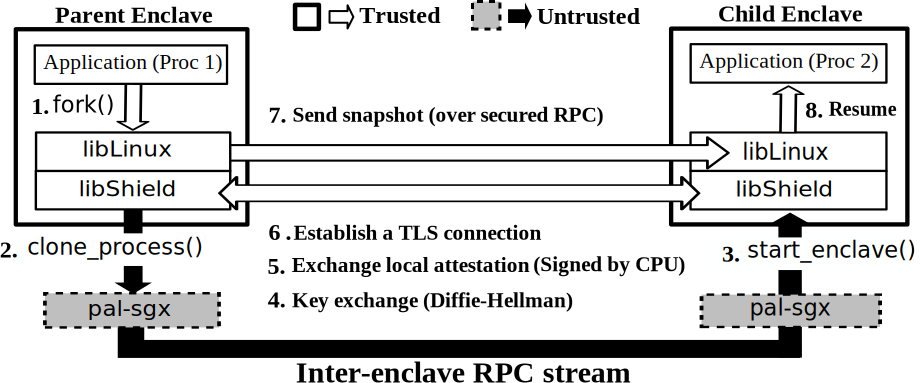
\includegraphics[width=5in]{graphene-sgx/figures/fork.pdf}
\footnotesize
\caption[Process creation in \sysname{}]
{Process creation in \sysname{}.
Numbers show the order of operations.
When a process forks, \sysname{} calls {\tt execve} system call
on the untrusted host,
to create a clean enclave with the same \libos{} image.
Then the two enclaves build up the mutual trust by
exchanging a session key, verifying attestation of each other,
and migrating the process snapshot from the parent.}
\label{fig:gsgx:fork}
\end{figure}

To secure process creation across enclaves,
\sysname{} is capable of building up the trust to newly launched enclaves,
through cooperation with an untrusted host.
Once a clean and trusted new enclave is launched,
The parent process will send a snapshot to the new one,
to create a clone of itself.
Snapshotting and migrating process states
is a feature robustly implemented and heavily used in \graphene{} \libos{},
of which we simply inherit the design.

When a process in \sysname{} forks,
because the parent and the child will be running the same binary,
both enclaves can simply be expected to have the same measurement.
To build up the trust, the two processes will open an encrypted channel
using a session key,
and exchange attestation generated by the processor.
Once both sides have confirmed the integrity of the other,
the parent process is safe to send its snapshot, encrypted, to the child
through the said channel.
The child process will restore the snapshot in its own enclave,
making it a clone of its parent.
The design of process creation in \sysname{} is shown as Figure~\ref{fig:fork}.

Forking in \sysname{} mainly defends against 3 types of attacks
from the untrusted host:

\begin{compactenum}

\item The host pretends to be the child enclave, to expose the process snapshot
sent from the parent.

\item The host pretends to be the parent enclave, to compromise the
child process using a malicious process snapshot.

\item The untrusted host becomes a man-in-the-middle, which bounces
encrypted messages between the child and parent enclaves, with session keys
negotiated with both sides.

\end{compactenum}

As described earlier, attacks 1 and 2 are prevented by mutual attestation
between the parent and the child,
and encrypting the channel for sending the snapshot.
The attestation signed by the processor proves that both entities communicating
are valid \sysname{} enclaves,
and encrypting the channel prevents the snapshot being eavesdropped or
counterfeited by the host.

To defend against attack 3 (the man-in-the-middle attack), we take advantage of
a user-customized 512-bit field
in the attestation structure generated and signed by \sgx{}.
This field is filled with a SHA-256 hash value of the agreed session key,
and the current enclave ID,
to prove that the attested enclave is the one who agrees on the key.

Once a parent enclave forks a child, by default the child must be trusted
to maintain its own security,
because the migrated snapshot discloses all information in the parent.
Unless the binary run in the parent enclave ensures
that no secrets is stored in the enclave memory at the time of snapshotting,
the parent enclave cannot simply drop the trust against the child.
For example, a pre-forked Apache web server may want to keep each worker
that responds to HTTP requests isolated,
to avoid being compromised by one attacked worker.
\graphene{} \libos{} provides an API for applications like Apache to explicitly
specify isolation to untrusted child processes.
\sysname{} inherits the ability of dynamic process isolation,
but developers are responsible for keeping confidential information
from the untrusted children.

\paragraph{Implementing {\tt execve}.}
Unlike {\tt fork}, {\tt execve} is used to
start processes with specified binaries, often different from the callers'.
When a thread in the process, either single-threaded or multi-threaded,
calls {\tt execve} in \sysname{},
\libos{} will migrate the calling thread to a new process,
with clean process states except opened files cloned from the parent.

The main challenge for implementing {\tt execve} is to
identify trusted binaries that can be loaded into new enclaves as child processes.
Consider the case where the parent process and its child shares
a multi-process abstraction (e.g., message queue).
Even if only the parent side is provisioned by the client, the child side
can still potentially compromise the secrets,
by exploiting vulnerabilities in the shared abstraction.
The trust between the parent and the child must be mutual,
unless the two enclaves are strictly isolated.

To identify binaries that can be trusted (either as parents or children)
during process creation,
\sysname{} requires each binary ported for an application,
to be shipped with a list of binaries that can be {\tt execve}'d,
and those that can be callers of {\tt execve} to the said binary.
Each binary in the list is identified by its measurement, which is mutually attested
between the parent and the child during process creation.
This list must be signed by a private key provided by the client,
while the public key must be included in the enclave measurement of the binary.

\subsection{Securing Inter-Process Coordination}
\label{sec:graphene:multiproc:ipc}

After process creation, a multi-process application often cooperate
through shared abstractions between processes,
such as signals or message queues.
For \libos{}, OS states for these shared abstractions must be shared
though inter-process coordination, for mainly two purposes.
First, for each abstraction, \libos{} needs to maintain the state
in one of its instances.
Second, \libos{} must maintain the namespace states to identify and locate the
abstraction states.

\graphene{} implements a wide range of multi-process abstractions and namespaces,
by passing messages over RPC streams among processes.
Such a design is perfect for porting multi-process applications to enclaves.
The benefit of sharing abstraction by RPC coordination are that
the enclaves will not have to share any memory to
coordinate abstraction states,
and the RPC streams can be secured by the enclaves instead of the host.

In \graphene{}, security isolation among multi-process abstractions,
regardless of their semantics,
are enforced by isolating the RPC streams used for coordination.
Unfortunately, \sysname{} cannot trust the host to faithfully isolate
the RPC streams.
Each enclave launched for an application must secure inter-process coordination
spontaneously, by only communicating to enclaves that it has attested
and exchanged secret keys with.
Because inter-process coordination is completely transparent
to the applications,
all information sent over RPC streams must be encrypted,
because \libos{} cannot determine whether the information may contain any secret.






\section{Implementation Details in \graphene{}}
\label{sec:graphene:impl}

\paragraph{Linux \pal{}.}
The majority of \pal{} calls are simple wrappers for similar Linux system calls, 
adding less than 100 LoC on average for translation between \pal{} and Linux abstractions.
The largest \pal{} calls are for exception handling, synchronization, and picoprocess
creation, which require multiple system calls and range from 500--800 LoC each.
Creating a new picoprocesses internally requires a {\tt vfork} and {\tt exec} of a clean 
application instance, and would be more efficiently implemented in the kernel.
Finally, the other major \pal{} components are an ELF loader (2 kLoC), headers (800 LoC),
and internal support code (2.3 kLoC).

\paragraph{Alternative \pal{} Ports.}
We prove the platform independence of \graphene{}
by porting \pal{} to \emph{FreeBSD}, \emph{OSX} and \emph{Windows}.
With the alternative host \pal{}, unmodified Linux binaries,
along with {\tt glibc} and {libLinux},
can be transparently run on the host.
For FreeBSD,
only 1.2 kLoC of the host \pal{} code need to be rewritten,
which are significantly less than FreeBSD Linux compatibility module (10.8 kLoC).
\pal{} components including ELF loader and internal support code can be shared by any \pal{} ports.

%\fix{We leave host \pal{} ports to non-unix OSes like Windows as future work,
%but previous works~\cite{porter11drawbridge,baumann13bascule} have already shown it feasible.}

\begin{table}[t!b!]
\footnotesize
\centering
\begin{tabular}{|l|rr|}
\hline
{\bf Component} & {\bf Lines} & ({\bf \% Changed})\\
\hline
GNU Library C ({\tt libc}, {\tt ld}, {\tt libdl}, {\tt libpthread}) & \libclines{} & $0.07\%$ \\
\hline
Linux Library OS ({\tt libLinux}) & 31,112 & \\
Linux host \pal{} & 11,644 & \\
Extra code for Linux \sgx{} host \pal{} & 9.354 & \\
% updated by Chia-Che on Oct. 10, 2013
\hline
%Storage Server & \fixmedp{XX} & \\
Reference monitor bootstrapper & \reflines{} & \\
Linux kernel reference monitor module ({\tt /dev/graphene}) & \sandboxmodlines{} & \\
Linux kernel IPC module ({\tt /dev/gipc}) & \gipclines{} & \\
\hline
\end{tabular}
\caption[Lines of code written or changed in \graphene{}]
{Lines of code written or changed to produce \graphene{}.  Applications and other libraries are unchanged.}
\label{tab:graphene:loc}
\end{table}


%% * most calls are a wrapper, \fixmedp{XX} LoC on average.
%% * Exception handling, sync, and process creation were harder (500-800 LoC each).  Process creation requires a clean instance (vfork+exec), would be simpler to implement in kernel.
%% * Other major components: ELF loader (2kLoC), headers(800 LoC), internal support code (2300 LoC)


%\fixmedp{Chia-Che, update LoC table}

\paragraph{Implementing Linux Personality.} 
%\fixmedp{Revisit the logical flow of these paragraphs}
The \graphene{} {\tt libLinux.so} implements a subset 
of the Linux system call API (currently \graphenesyscalls{} calls)
using only the \pal{} ABI to interact with the host.
We note that Linux exports a very long tail of infrequently used calls.
%applications.
A rough analysis of this tail indicates roughly 100 additional calls that can be implemented
with the existing \pal{} ABI and coordination framework, less than 10 administrative calls that will not make sense to expose to 
an application, such as loading a kernel module or rebooting the system, and roughly 54 that will require 
\pal{} extensions to meaningfully implement, such as controlling scheduling,
NUMA placement, I/O privilege, and shared memory.
In the last category of system calls, the degree to which actual host details should be exported versus emulated is debatable.

%We believe represent the most commonly used system calls.
%When an application requests a call or argument that {\tt libLinux.so} does not implement,
%the picoprocess exits with a distinct error message. 
Each time we have tested \graphene{} with a new application, the number of extra system calls
required has dropped---most recently we only added 4 calls
(namely, epoll\_create, epoll\_wait, semget and semop)
to support the Apache web server.
Thus, we believe \graphene{} implements a representative sample of Linux calls.

%such as {\tt sched\_setparam}, which manipulates scheduler-specific
%parameters or 
%{\tt uselib}, which has been abandoned 
%in {\tt glibc} version 2 in favor of a user-space dynamic linker.
%We do not plan to implement administrative interfaces, such as {\tt reboot}.
%The growth in the set of supported system calls has been driven by 
%the requirements of new applications we use to exercise \graphene{}, and has been 
%slowing considerably over time.

%directly to guests, and thus will not implement them in {\tt libLinux.so}.

% dp: :(
\begin{comment}
Most {\tt libLinux.so} code reimplements
Linux kernel functionality.  We found it expedient to 
read the Linux source in order to understand its behavior and then reimplement 
that behavior on the \pal{} ABI in most cases.
In some cases, such as the file caching code,
%directory entry (dentry) cache, 
we refactored code directly from the Linux kernel.
%% In these cases, we simplified data structures to only include data
%% we needed for a single application, and to hook in with other 
%% {\tt libLinux} subsystems.
%% An interesting direction for future work would identify techniques
%% to automatically import larger swaths of Linux kernel code, facilitating
%% adoption of new features and bugfixes.
\end{comment}

In order to use {\tt libLinux.so}, we modified \libclines{} lines of {\tt glibc} to replace 
system instructions with function calls into {\tt lib\-Linux.so},
and to cooperatively manage thread-local storage with {\tt libLinux.so} (Table~\ref{tab:graphene:loc}).

%All totaled, we only needed to modify \libclines{} lines of glibc source code to redirect all 
%system calls to {\tt libLinux} 

\begin{comment}
\vspace{5pt}
\noindent{\bf ABI Extensions.~}
\graphene{} extends the Drawbridge ABI with 9 additional \pal{} calls.
As discussed above, one creates a new sandbox, and 
5 additional calls were added for IPC.
We also add 3 calls to manage x86 segmentation registers
and exceptions (Bascule~\cite{baumann13bascule} adds
similar extensions).
\end{comment}

\paragraph{Synchronization.} Perhaps surprisingly, implementing Linux
synchronization appears substantially easier than Windows synchronization, 
as {\tt libLinux} did not require all of the various
synchronization ABIs provided by Drawbridge.
We believe the reason for this is that Linux has consolidated 
all user-level synchronization primitives to use futexes~\cite{franke02futex},
which are essentially kernel-level wait queues.
%In Windows parlance, this is simply an Event associated with a virtual address.
%Thus, our effort implementing synchronization was relatively straightforward.

%\subsection{Linux Host \pal{}}
\label{sec:linux:pal}

\begin{comment}
The Platform Adaptation Layer (\pal{}) exports a generic host kernel interface to the guest, summarized in Table~\ref{tab:abi}.
Our Linux host \pal{} consists of a user library and a small Linux kernel module.
Our \pal{} library is implemented using  \nativecalls{} native Linux system calls.
%The specific division of labor between the host kernel and user library
%could be different in another implementation.
%We currently implement only a Linux host \pal{}.  
If a different host kernel implements the same \pal{} ABI,
{\tt libLinux.so} and all binaries
should execute without modification.


%How we connect the shim to the \pal{}?  Expedient to hack the loader to add it to the link tables.  Describe.  
%-Dynamically linked, included in loader (ld.so can't mmap the \pal{}; conceptually should be mapped by the OS)
%-imported by libc
%-- Does a new binary type require kernel mods?  If so, make claim about unmod host
%-- conceptual leakage by tightly coupling pal and loader; pal should be provided by the host OS
% validated that no other native system calls
%% were being issued by application directly to the host kernel with {\tt strace} 
%% and by disassembling application binaries.
%% In future work, we will replace the native Linux system call table 
%% with a restricted system call (or hyper call) table to host.
%potentially migrating much of the \pal{} implementation into the host kernel.

We selected the Drawbridge ABI~\cite{porter11drawbridge} as a starting point for the \sysname{} ABI,
because it strikes a good balance between host platform independence 
and avoiding duplicate functionality.
In porting Linux to the Drawbridge ABI, which was designed for a Windows library OS,
we strove to only add additional interfaces when otherwise unavoidable for
functionality or performance.
In some cases, revisiting the Drawbridge design choices 
could simplify {\tt libLinux},
but we wanted to understand how well the Drawbridge design generalizes to other guests, 
without undermining its simplicity.
\end{comment}

%We note that we reimplemented the Drawbridge ABI according to the published description and 
%expect that both systems two could be interoperable
%with a modest amount of reconciliation effort where the published specification is ambiguous;
%because Drawbridge is not publicly available, we cannot test interoperability of the library OSes.


\begin{comment}

\noindent \sysname{} requires  the following additional \pal{} calls:
\begin{compactenum}
%% dp: I think these are the key ones
%\item \fixmedp{What is missing here}
% What is: DkThreadSelf - is this necessary?  
% DkThreadPrivate
\item {\tt DkSetSegmentRegister} --- Set the optional segmentation
  register values ({\tt fs} and {\tt gs} on {\tt x86\_64}).  This functionality 
  is required
  for thread-local storage, which is initialized in user-space
  by the Linux loader.
  The Windows kernel initializes these registers before process execution begins, 
  obviating the need to initialize them from user-space.
  We further note that different OSes use these registers differently
  (e.g., 32-bit Windows uses {\tt gs} for TLS, whereas Linux and 64-bit Windows use {\tt fs} for TLS),
  therefore management of these registers should be in the domain of the guest.
\item {\tt DkSetExceptionHandler} --- Register a callback for a hardware exception, 
  such as a divide by zero error or segmentation fault.  This is roughly analogous 
  to a software emulated interrupt descriptor table (IDT).  
  %In future work,
  %we will adopt techniques proposed previously to send processor exceptions directly to the guest~\cite{belay12dune}.
\item {\tt DkExceptionReturn} --- Returns from an exception back to the host kernel.
   %% In our current design, the host kernel is responsible for returning control flow 
   %% back to the thread that was running when an exception occurs.
   %% Alternatively, the \sysname{} ABI could require exception delivery to include
   %% a register trapframe sufficient to resume execution directly in user space.
% Async upcall; return necessary?
%\fixmetsai{I am not sure how to put this, but the design of Return is to leave \pal{} independent from its host semantic
%%%    With the extra call, guests no long need to worry about the stack structure that
%%%    \pal{} created at exception handling. For example, \pal{} might put extra objects on stack, or use an
%%% alternative stack. These design will make the guest crash while trying to return.
\item {\tt DkCreatePhysicalMemoryChannel}, {\tt Dk\-Physical\-Memory\-Send}, and {\tt Dk\-Physical\-Memory\-Recv} --- These calls mark a set of pages in the sender's address space as copy-on-write (COW) 
  and then map the pages as COW in the receiver's address space.
  Although these calls are not strictly required, as
  data can be sent over a stream, we found the ability to exchange 
  large quantities of data efficiently to be an important 
  performance optimization for {\tt fork}  (\S\ref{sec:fork}).

\item {\tt DkHandleSend}, {\tt DkHandleRecv} --- Send a stream 
  handle out-of-band to another guest in the same sandbox.
  This is used to establish connections both for namespace
  coordination (\S\ref{sec:namespaces}) and 
  handle inheritance (\S\ref{sec:fork}).
  

%  This mechanism required extending the Linux kernel with a \gipclines{} line module,
%  discussed below.
%  This module does not require any kernel changes or recompilation.
  
\end{compactenum}
\fixmedp{isolate pal call?}

%%% Extra \pal{} calls we needed.  Describe issues. \fixmedp{Can I get a list?}
%%% -mutex (don)
%%% -cv (don)
%%% -IPC physical memory calls send/recv
%%% -set\_thread\_private - sets segmentation registers for TLS
%%% -synchronous event - sets hardware exception handlers + OS callbacks (seg fault, div zero, external kill, async io, interrupts, etc.) roughly analogous to idt
%%% -system initialize - get control block address for checkpointing/etc. - avoids assumptions about address space layout

\paragraph{Fast bulk data movement.} 
We extend the Linux host kernel with a
fast bulk IPC mechanism.  The bulk IPC mechanism does a 
copy-on-write (COW) data transfer between two guests.
A sender designates virtual pages to send to 
the receiver;
these pages are then placed in a first-in-first-out queue.
The receiver then requests these pages be mapped into its address space,
optionally providing a target virtual address (similar to {\tt mmap}).
The sent pages need not be virtually contiguous, 
allowing the guest to efficiently gather and send scattered pages.
%This is useful for implementing guest-managed page caches.

\sysname{} uses bulk IPC in conjunction with control
messages on a byte stream; 
the byte stream communicates the expected meaning and ordering 
of the corresponding bulk data transfer.
In the common case, these physical pages are quickly shared between
two processes, minimizing data copying
for user-level implementations of system calls like {\tt fork}.
%The CAS server commonly
%unmaps sent pages, which will reduce the page reference 
%count to one and eliminate the need to copy the page on a 
%on a write fault in the receiver.

Our bulk IPC module is \gipclines{} lines of code, 
runs on multiple versions of Linux (2.6 and 3 series kernels), and
does not require
Linux kernel changes or recompilation.
\end{comment}

%% dp: So sad, but something has to go
\begin{comment}
\paragraph{Efficient creation of clean processes.}
We implement a process creation ABI in the host 
that only creates 
clean child picoprocesses that do not inherit memory mappings
or open file handles from the parent, similar to booting another VM.
This design choice strengthens security isolation.

Linux does not provide a process creation mechanism other than {\tt fork()} (or variants, such as {\tt clone()}).
Thus, the \pal{} is must implement this abstraction on Linux processes.
A simple implementation of {\tt Dk\-Pro\-cess\-Create()} would {\tt fork} 
a new process,
clean the open file handles, and then {\tt exec} the new binary.
This simple implementation of process creation
wastes work implementing an ABI that will always {\tt exec()} a clean process.
%%% The {\tt fork-exec} approach bring unwanted overhead to {\tt fork} and {\tt execve}
%%% system call. Compare to the native system calls, reloading the whole \sysname{}
%%% system causes duplicated works such as parsing manifests and linking libraries.

The \pal{} optimizes process creation by forking 
a newly launched picoprocess after initializing all of the operating system state,
but before starting any application-specific work, such as calling the ELF loader.
Dune leverages a similar optimization to efficiently create
isolated threads in the Wedge case study~\cite{belay12dune}.
The checkpoint process is not visible to the application.
This checkpoint listens for a message from the \pal{} to 
fork itself in order to create a clean child.

Because new processes are created by forking the checkpoint process,
as a guest creates children, they are actually siblings
from the perspective of the host kernel.
The guest implements the abstraction of a Linux process tree inside the library OS.

This checkpointing strategy works well even if the application 
requests that the child load a different application
binary, because the checkpoint is taken before {\tt ld.so} links in the application.
In a simple microbenchmark,
this checkpointing strategy improved picoprocess creation time
 a factor of two.

%This approach is \fixmedp{XX\%} faster than simply {\tt exec}-ing 
%the \pal{} in the child to clean up parent state.

%%% This strategy of checkpointing the process manager allows \sysname{} to quickly 
%%% create clean child processes in user-space on an unmodified Linux kernel.  
%%% In a simple microbenchmark,
%%% this pre-forking strategy improved {\tt DkProcessCreate} time
%%% by a factor of two.


\end{comment}




%\input{examples}
\declarecommand{\sysname}{\graphene{}}
\declarecommand{\pal}{PAL}
\declarecommand{\syscalls}{131}
\declarecommand{\palcalls}{43}
\declarecommand{\nativecalls}{50}
\declarecommand{\gipclines}{1,131}
\declarecommand{\sandboxmodlines}{888}
\declarecommand{\reflines}{3,568}
\declarecommand{\libclines}{606}
\declarecommand{\interfacenum}{41}
\declarecommand{\light}{lighttpd}
\declarecommand{\gcc}{gcc}
\declarecommand{\lmbench}{LMbench}
\declarecommand{\ab}{ApacheBench}
\declarecommand{\busy}{Bash}
\declarecommand{\skylake}{Skylake}

\chapter{Evaluation}
\label{chap:eval}
\chapter{Related Works}
\label{chap:related}

\makeatletter
\def\input@path{{related/}}
\makeatother
\graphicspath{{related/figures/}}

This chapter describes the formal definition of the \graphene{} host ABI.

\section{Basic Definitions}

The \graphene{} host ABI defines a set of {\em functions}, similar to the API of UNIX or POSIX.
The functions are directly called by the library OS, along with the arguments given either in the registers or on the stack.
A host-specific \graphene{} loader is responsible for resolving the linking, from the library OS to the host ABI.
\section{Library OSes and virtualization}





\paragraph{Previous library OSes.}
Previous library OSes~\citep{porter11drawbridge,xax,unikernels,baumann13bascule,osv}
focus on running single-process applications
in a \picoproc{} or a unikernel
for verious reasons including compatibility and security isolation.
%to support coordination abstractions required 
%for multi-process applications, such as shell scripts.
Bascule~\citep{baumann13bascule} implements a Linux library OS on a variant of the Drawbridge ABI,
but does not include support for multi-process abstractions such as signals or copy-on-write fork.
The Bascule Linux library OS also implements fewer Linux system calls than Graphene, missing
features such as signals.
Bascule demonstrates a complementary facility to Graphene's multi-process support: composable library OS extensions, 
such as speculation and record/replay.
OSv is a recent open-source, % project to design and implement a 
single-process 
library OS to support a managed language runtime, such as Java, on a bare-metal hypervisor~\citep{osv}.


A number of recent projects have provided a minimal, isolated environment
for web applications to download and execute native code~\citep{nacl,xax,howell13refactoring,gazelle,atlantis}.
The term ``picoprocess'' is adopted from some of these designs, and they share 
the goal of pushing system complexity out of the kernel and into the application.
%%% Despite these common design themes, the motivations
%%% for these projects varies widely, including
%%% robustly enforcing browser policy\citep{gazelle};
%%% ensuring that a web page is compatible with the JavaScript, CSS, and other interpreters in the browser~\citep{atlantis};
%%% and simply the ability to push code from the data center onto the client where it makes 
%%% sense~\citep{nacl, embassies, howell13refactoring}.
Unlike a library OS, these systems
generally sacrifice the ability to execute unmodified application code, 
eliminate common UNIX multi-process functionality (e.g., fork), or both.


The term library OS also refers to an older generation of research
focused on tailoring hardware management heuristics 
to individual application needs~\citep{kaashoek97exokernel,anderson92libos,cheriton94cache,leslie96nemesis,libra},
whereas newer library OSes, including Graphene, focus
on providing application compatibility
across different hosts without dragging along an entire legacy OS.
A common thread among all libOSes is moving functionality from the kernel
into applications and reducing the TCB size or attack surface.
Kaashoek et al.~\citep{kaashoek97exokernel} identify multi-processing as a problem for an Exokernel libOS,
and implemented some shared OS abstractions.
The Exokernel's sharing designs rely on shared memory rather than byte streams,
and would not work on recent libOSes,
nor will they facilitate dynamically sandboxing two processes.

%% In moving services out of the kernel and into user libraries our design resembles a microkernel~\citep{liedtke95sosp, Baron:1985:MOE}.
%% %liedtke93sosp,liedtke95sosp, Baron:1985:MOE, Jones:1986:MMK, Rashid:1987:RAM}.
%% An important distinction is that
%% microkernels generally centralize system services in a single trusted daemon,
%% whereas Graphene distributes management of coordination APIs among
%% cooperating guests.

\begin{comment}
Dune~\citep{belay12dune} %merges the concept of a process and VM,
leverages virtualization hardware 
to allow an application
to safely manage privileged CPU features
such as page tables and interrupts.
%Dune leverages virtualization hardware  to safely 
%isolate privileged hardware access within a process.
Dune's goals are complimentary to ours; we expect that
certain aspects of the PAL implementation would be simplified on Dune.
\end{comment}

User Mode Linux~\citep{user-mode-linux} (UML) executes a Linux kernel inside a process
by replacing  architecture-specific code with 
code 
that uses Linux host system calls. % to emulate this functionality.
%Because UML runs a complete Linux kernel and multiple processes,
%it is effectively
UML is best described as  an alternative approach to paravirtualization~\citep{barham03xen},
and, unlike a library OS, does not deduplicate functionality.


\paragraph{Virtualization.}
Recent library OSes, including Graphene,
search for a better
division of labor between the host kernel and guests.
Paravirtualized VMs attempt to move away from modeling specific hardware designs in software
toward a more virtualization-friendly hardware model~\citep{barham03xen,whitaker02denali, eiraku09outsourcing}.
Library OSes can be viewed as extreme paravirtualization---attempting
to find the most ideal interface between guest and host. %abstractions of hardware without also baking-in host semantics.



\paragraph{Distributed coordination.}
Distributed operating systems,such as LOCUS~\citep{locus83sosp,fleisch86locus}, Amoeba~\citep{mullender90amoeba,cheriton89naming} and  
Athena~\citep{champine90athena} required a consistent namespace for process identifiers and other IPC abstractions
across physical machines.
%A key requirement for naming in a distributed OS is network transparency---that the name should be independent of the physical placement of an object in the system.
Like microkernels, these systems generally centralize all management in a single, system-wide service.
%For instance, Amoeba has a single session server that allocates process identifiers.
%This system service may be replicated or partitioned for improved performance on a large network or to
%divide management responsibility across administrative domains~\citep{cheriton89naming}.
%Each Graphene guest also needs to coordinate naming of Unix abstractions, such as processes or System V IPC keys.
%Although Graphene draws some inspiration from these distributed OSes, 
%Graphene's goals and usage model are different, and 
Rote adoption of a central name service does not meet our goals
of security isolation and host independence.

Several aspects of the Graphene host kernel ABI are similar to the
Plan 9 design~\citep{pike90plan9}, including the unioned view of the host file system
and the inter-picoprocess byte stream.
Plan 9 demonstrates how to implement this host kernel ABI,
whereas Graphene uses a similar ABI 
to encapsulate multi-process coordination 
in the libOS.

%% or coordinating coordinate a distributed file system
%% across multiple workstations,
%% but rather to demonstrate how it can be leveraged to 
%% implement a more efficient guest library OS. instance, Plan 9 uses the 9P protocol to coordinate a distributed file system
%% across multiple workstations. In contrast, Graphene uses streams




Barrelfish~\citep{baumann09barrelfish} argues that multi-core scaling is best served 
by replicating shared kernel abstractions at every core, and using message passing 
to coordinate updates at each replica, as opposed to using cache coherence to update a shared data structure.  
Barrelfish is a new OS; in contrast,
Cerberus~\citep{song11eurosys} applies similar ideas to coordinate abstractions
across multiple Linux VMs running on Xen.
%Cerberus coordinates a unified view of the process tree, file system, network card,
%and the address space when threads run on separate cores---forwarding 
%some system calls to other kernels as remote procedure calls.
In order for a library OS to provide multi-process abstractions, 
Graphene must solve some similar problems, but innovates by
replicating additional classes of coordination abstractions, such as System V IPC,
and facilitates dynamic sandboxing.
%and optimizes performance through 
%techniques such as lazy discovery.
The focus of this paper is not on multi-core scalability, but on security isolation and compatibility with legacy, multi-process applications.
That said, we expect that systems like Barrelfish~\citep{baumann09barrelfish} 
could leverage our implementation techniques to efficiently 
construct higher-level OS abstractions, such as System V IPC and signals.

%% We note that several recent projects argue that multi-core scalability 
%% is enhanced by eschewing cache coherence and shared data structures, 
%% in favor of a similar 
%% design which
%% replicates state across cores
%% {\em within an OS kernel}~\citep{baumann09barrelfish} or {\em across legacy guest OSes}~\citep{song11eurosys}.
%% The focus of this paper is not on multi-core scalability, but on security isolation and compatibility with legacy, multi-process applications.
%% That said, we expect that systems like Barrelfish~\citep{baumann09barrelfish} 
%% could leverage our implementation techniques to efficiently 
%% construct higher-level OS abstractions, such as System V IPC and signals.

L3 introduced a ``clans and chiefs'' model of IPC redirection, in which IPC to
a non-sibling process was validated by a the parent (``chief'') before a message could leave the clan~\citep{liedtke92clans}.
%This model was primarily used to enforce access control on system abstractions,
%and abandoned for capabilities on kernel objects in L4
Although this model was abandoned as cumbersome for general-purpose access control~\citep{elphinstone13microkernels},
the Graphene sandbox design observes
that a stricter variation is a natural fit
for security isolation among multi-process applications.

Cerberus focuses on replicating lower-level state, such as process address spaces
which Graphene leaves in the host kernel.
As a result, the performance characteristics are different.
Although this comparison is rough, 
we replicated their test of ping-ponging 1000 
{\tt SIGUSR1} signals and compare the ratio to their reported data, 
albeit with different hardware and our baseline kernel is newer 
(3.2 vs 2.6.18).  
When signals are sent inside of a single guest on Graphene, they are {\em faster}
by 79\%, whereas performance drops by a 5.5--18$\times$ on Cerberus.
When passing signals across coordinating guests both approaches are competitive:
Graphene's cross-process signal delivery is 4.6$\times$ slower than native, whereas Cerberus ranges from 
3.3--11.3$\times$ slower, depending on the hardware.


%% For instance, Graphene guests may require a mixture of isolated and shared namespaces.
%% Moreover, Graphene naming must support dynamic detachment of one guest from a confederation of other guests.
%% Our work contributes  an implementation of distributed naming inside the library OS, facilitating security isolation, 
%% and application-transparent detachment.

\paragraph{Migration and security isolation.}
Researchers have added checkpoint and migration support to Linux~\citep{linux-cr}
by serializing kernel data structures to a file
and reloading them later.  
This introduces several challenges, including
security concerns of loading data structures into the OS kernel from a potentially 
untrusted source.
%, as well as significant engineering and maintenance effort.
In contrast, Graphene checkpoint/restore 
%on a simple host ABI
requires little more than a guest memory dump.
%The host state can be easily restricted by a sandbox.

%% supports migration of one or more process across
%% hosts with the same kernel.
%% To maintain consistency of namespace and resource throughout migration,
%% Zap provides a thin virtualization layer upon which
%% application can have the same virtualized and conflict-free view of system.
%% To simplify process dependency that complicates migration, Zap migrates
%% processes in the unit of Pods, a container with virtualized namespace,
%% memory checkpoints and private file system. 

%Docker - http://www.docker.io/ - really looks like it just automates creation of a minimal hard drive

OS-based virtualization, such as 
Linux VServer~\citep{vserver},  containers~\citep{bhattiprolu08containers},
and Solaris Zones~\citep{price04zones},
implement security isolation by maintaining multiple copies of kernel data structures,
such as the process tree,
in the host kernel's address space.
In order to facilitate sandboxing, 
Linux has added support for launching single processes
with isolated views of namespaces, including process IDs and network interfaces~\citep{lwn-namespaces}.
FreeBSD jails apply a similar approach to augment an isolated {\tt chroot} environment
with other isolated namespaces, including the network and hostname~\citep{jails}.
Similarly, Zap~\citep{osman02zap} migrates groups of process, called a Pod,
which includes a thin layer virtualizing system resource names.
In these approaches, all guests must use the same OS API, and the host kernel
still exposes hundreds of system calls to all guests.
Library OSes move these data structures into the guest, enabling
a range of personalities to run on a single guest and limiting the attack surface
of the host.


Shuttle~\citep{shan12shuttle} permits selective violations of strict isolation
to communicate with host services 
under OS-based virtualization.
For example, collaborating applications may communicate using the Windows Common Object Model (COM);
Shuttle develops a model to permit access to the host COM service.
%Windows guest applications 
%may rely on the host's Service Control Manager
%for certain functionality, and this functionality cannot be replicated inside of each guest.
%Similarly, some collaborating applications may 
Rather than attempting to secure host services,
Graphene moves these services out of the host
and into collaborating guests.


%From an API perspective, this is similar to Graphene's isolation.  
%This approach requires all applications to run on the same host kernel,
%and 
%However, these approaches are implemented in the same address space 
%as the host kernel and still expose a wide attack surface area.  
%The library OS
%approach moves much of this attack surface area out of the kernel and into the guest.

\section{Graphene on SGX}
\label{sec:eval:sgx}

%This section will shows the evaluation results of the \graphenesgx{} framework,
%in term of performance, security, and compatibility to Linux.

%\subsection{Performance Evaluation}
\label{sec:eval:perf}


%We evaluate the performance overheads on running unmodified Linux applications
%on SGX.
%Unlike the existing \sgx{} shielding systems which focuses on cloud-based systems or microservices,
\graphenesgx{} is designed to be general-purpose, supporting a broad range of
server and command-line applications. 
%, including both server and desktop workloads.
%\fixmedp{I wouldn't really call gcc or R ``desktop''}
\fixme{get rid of the part that we need to compile source code}
We thus evaluate performance overheads of unmodified Linux applications, using binaries 
from an Ubuntu installation.
%, or,
%in the case of Apache, Lighttpd, and NGINX,
%compiled from original source code using the default configurations.}
%(Apache, Lighttpd, and NGINX are compiled from source).} %\fixmedp{which apps are compiled?}
Depending on the workload, we measure application throughput or latency.
%According to the types of workloads, we design experiments to evaluate whether \graphenesgx{} can support applications with acceptable throughput or latency.

%All applications in our experiments are real, unmodified Linux applications,
%either directly taken from a disk with Ubuntu installation,
%or compiled using the default configuration given by the developers.
%No source code modification or change of compilation environment is required in the experiments.
%In our experiments, we either test on application binaries taken off-the-shelf from the Ubuntu {\tt APT} repositories,
%or applications that are built from the default configurations
%provided by the developers.
%Either source code modification or adjustment of the compilation environment is avoided in the setup of experiments.
%Our evaluation simulates the realistic results of running unmodified Linux applications in \graphenesgx{}.
%running Linux COTS applications on commodity hardware.

In order to differentiate SGX-specific overheads 
from Graphene overheads,
%, which also
%runs on a Linux host without SGX, 
we use both
Linux processes and \graphene{} on a Linux host without SGX as baselines
for comparison.
%Since a large portion of the \libos{} design is inherited from the \graphene{} \libos{},
%the performance impact of adopting \graphenesgx{} is largely affected by the design choices made in \graphene{}.
%In order to show the performance impact of \graphenesgx{} over \graphene{}, we use both native Linux and \graphene{} on a Linux host as the baselines for comparison.
Note that \graphene{} includes two optional kernel extensions:
one that creates a reference monitor to protect the host kernel from 
the library OS, and one that optimizes fork by 
with copy-on-write for large (page-sized) RPC messages.
%implementing a multi-page RPC
%abstraction.
Neither of these extensions are currently supported in \graphenesgx{}.
%so we measure baseline Graphene with these disabled.
% can be optionally run with a reference monitor for security isolation, and a bulk IPC abstraction for fork optimization.
%Since neither of the features is ported in \graphenesgx{},
%we mostly compare \graphenesgx{} to \graphene{} with these two features disabled,
%to show a more meaningful comparison.

% Put figures at the front
\begin{figure*}[t!]
\centering

\begin{minipage}{.3\textwidth}
\centering
\footnotesize
\includegraphics[width=\linewidth]{sgx/lighttpd-throughput-latency}\\
{\bf (a) Lighttpd (25 threads)}
\end{minipage}
\begin{minipage}{.3\textwidth}
\centering
\footnotesize
\includegraphics[width=\linewidth]{sgx/apache-throughput-latency}\\
{\bf (b) Apache (5 processes)}
\end{minipage}
\begin{minipage}{.3\textwidth}
\centering
\footnotesize
\includegraphics[width=\linewidth]{sgx/nginx-throughput-latency}\\
{\bf (c) NGINX (event-driven)}
\end{minipage}

\caption{Throughput versus latency of web server workloads, including Lighttpd, Apache, and NGINX, on native Linux, \graphene{}, and \graphenesgx{}.
We use an ApacheBench client to gradually increase load, and plot
throughput versus latency at each point.  Lower and further right
is better.
%\fixmedp{RB: Add another sentence or two to explain what the experiment is and how to interpret} }
}
\label{fig:server-throughput-latency}
\end{figure*}


\fixmedp{RA asks for a limitations section; I don't think we should do this, but the expensive stuff (events, fork, open) we should add as much as we can about what, if anything,  can be done about it, and what can't without more hardware}

\paragraph{Experimental setup.}

We use a Dell Optiplex 790 Small-Form Desktop,
with a 4-core 3.20 GHz Intel Core i5-6500 CPU (no hyper-threading, with 6MB cache),
8 GB RAM, and a 512GB, 7200 RPM SATA disk.
%We disable SpeedStep and TurboBoost to prevent interference.
The host OS is Ubuntu 16.04.4 LTS, with Linux kernel 4.4.0-21.
Each machine uses a 1Gbps Ethernet card connected to a dedicated local network.
We use version 1.8 of 
the Intel \sgx{} Linux SDK~\cite{intel-sgx-linux-sdk} and driver~\cite{intel-sgx-linux-driver}.
%We measure version 0.4beta of \graphene{}.

%Adding more detail of KVM environment
%Unless otherwise noted, \graphenesgx{} measurements include the Phosphor instrumentation.

\subsection{Server applications}

One deployment model for SGX is to host network services
on an untrusted cloud provider's hardware.
%To measure this case, 
We measure three widely-used Linux web servers, including {\bf Lighttpd}~\cite{lighttpd} (v1.4.35), {\bf Apache}~\cite{apache} (v2.4.18), and {\bf NGINX}~\cite{nginx} (v1.10).
%, to evaluate the performance of server-type workloads in \graphenesgx{}.
%These applications are all sophisticated, non-trivial workloads, and are constantly being used for commercial purposes.
%We test these applications to evaluating significantly different execution patterns, to benchmark the performance of \graphenesgx{} under each circumstances.
%Also, we do not explicitly configure these servers to secure their payloads using the HTTPS protocol.\fixme{if have time, maybe try again with HTTPS}
For each workload, we use ApacheBench~\cite{apachebench} to download the web pages on a separate machine.
%\edit{over Gigabit LAN}. %\fixmedp{more specific?}
%across a high-speed \fixmedp{Can you say
%more specifically the specs, like 10 GBps or whatever; also, if this is the same vlan, I might just describe this as being on a LAN, minimizing interference} University network.
The concurrency of ApacheBench is gradually increased during the experiment, to test the both the per-request latency and the overall throughput of the server.
Figure~\ref{fig:server-throughput-latency} shows the throughput versus latency of these server applications
in \graphenesgx{}, \graphene{} and Linux. 
Each workload is discussed below.

{\bf Lighttpd}~\cite{lighttpd} is a web server designed to be light-weight, yet robust enough for commercial uses. 
Lighttpd is multi-threaded; we test with 25 threads to process HTTP requests. 
By default, Lighttpd uses the \syscall{epoll\_wait} system call to poll listening sockets.
At peak throughput and load,  both \graphene{} and \graphenesgx{} have marginal overhead on either latency or throughput of the Lighttpd server.
The overheads of \graphene{} are more apparent when the system
is more lightly loaded, at 
%When Lighttpd is not overloaded, \graphenesgx{} causes 
15--35\% higher response time, or 13--26\% lower throughput. 
Without SGX, \graphene{} induces 
11--15\% higher latency or 13-17\% lower throughput over Linux;
the remaining overheads are attributable to SGX---either hardware or our OS shield.
%platform adaptation layer (PAL) code.

%\fixmedp{Some more detailed analysis would be nice.}
%Only part of this overhead is contributed by the library OS implementation, since using \graphene{} without \sgx{} causes only 

%\fixmedp{Why did you comment this out?  Let's discuss: Does it really make sense to have two points at the same  x-axis value?  Perhaps the axes should be inverted?  I'm not really sure about the methodology, but something about the line doubling back on itself seems wrong.  Maybe you want to separate these and show throughput vs. load, and a CDF of latencies?}


{\bf Apache}~\cite{apache} is one of the most popular production web servers. We test Apache using 5 preforked worker processes to service HTTP requests,
in order to 
to evaluate the efficiency of \graphenesgx{} across enclaves.
%n server, 
%In the experiment, the Apache server creates 5 preforked processes which coordinate on processing HTTP requests.
This application uses IPC extensively---the preforked processes of a server use a System V semaphore to synchronize on each connection.
%When receiving a connection, the preforked processes of Apache will coordinate among themselves using the system V IPC semaphores.
Regardless of the workload, the response time on \graphenesgx{} is 12--35\% higher than Linux, due to the overhead of coordination across enclaves over encrypted RPC streams.
The peak throughput achieved by Apache running in \graphenesgx{} is 26\% lower than running in Linux.
In this workload, most of the overheads are SGX-specific, such as exiting enclaves when accessing the RPC, as non-SGX Graphene
has only 2--8\% overhead compared to Linux.

%The enclave restriction \fixmedp{Huh?} is the main contributor to this overhead, as \graphene{} generally only causes 2--8\% overhead.

%\fixmedp{Check the lightttp graph; the lines are right on top of each other, and dont' look 22\% apart to me.  Some of this may be the scale of the y axis}

{\bf NGINX}~\cite{nginx} is a relatively new web server designed for high programmability, for as a building block to implement different services.
Unlike the other two web servers, NGINX is event-driven and mostly configured as single-threaded.
%When running as a simple HTTP server, NGINX uses an event-driven model instead of multi-threading/multi-processing to handle incoming requests.
\graphenesgx{} currently only supports synchronous I/O at the enclave boundary,
and so, under load, it cannot as effectively overlap I/O and computation
as other systems that have batched and asynchronous system calls.
%Asynchronous system calls and events in general are less mature features of
%\graphenesgx{}, and, 
Once sufficiently loaded, NGINX on both \graphene{} and \graphenesgx{} 
performs worse than in a  Linux process. % once sufficiently loaded.
%We observe that both \graphene{} and \graphenesgx{} tend to perform poorly in an event-driven server.
The peak throughput of \graphenesgx{} is 1.5$\times$ lower than Linux;
without SGX, Graphene only reaches 79\% of Linux's peak throughput.
%\fixmedp{Maybe shout out to eleos, or cite other work}
We expect that using tools like Eleos~\cite{orenbach17eleos} to reduce exits
would help this workload; in future work, we will improve
asynchronous I/O in \graphenesgx{}.

%\graphenesgx{} causes 17--90\% more response time when the server is not overloaded,
%but up to 1.5$\times$ at the peak throughput.
%If we compare the peak throughput with native Linux, \graphenesgx{} is 70\% less.
%\graphene{} also suffers the same performance pattern, as the throughput drops dramatically after reaching 79\% of the peak throughput of NGINX in Linux.
%The reason of the slowdown is that the host interface of \graphene{} and \graphenesgx{} only supports synchronous IO, so implementing asynchronous IO will be less efficient. This limitation is a trade-off to the portability of \graphene{}.
%\fixmedp{Didn't get the portability point; please spell out what you meant, if important}

\begin{figure*}[t!]
\centering

\begin{minipage}{.4\textwidth}
\centering
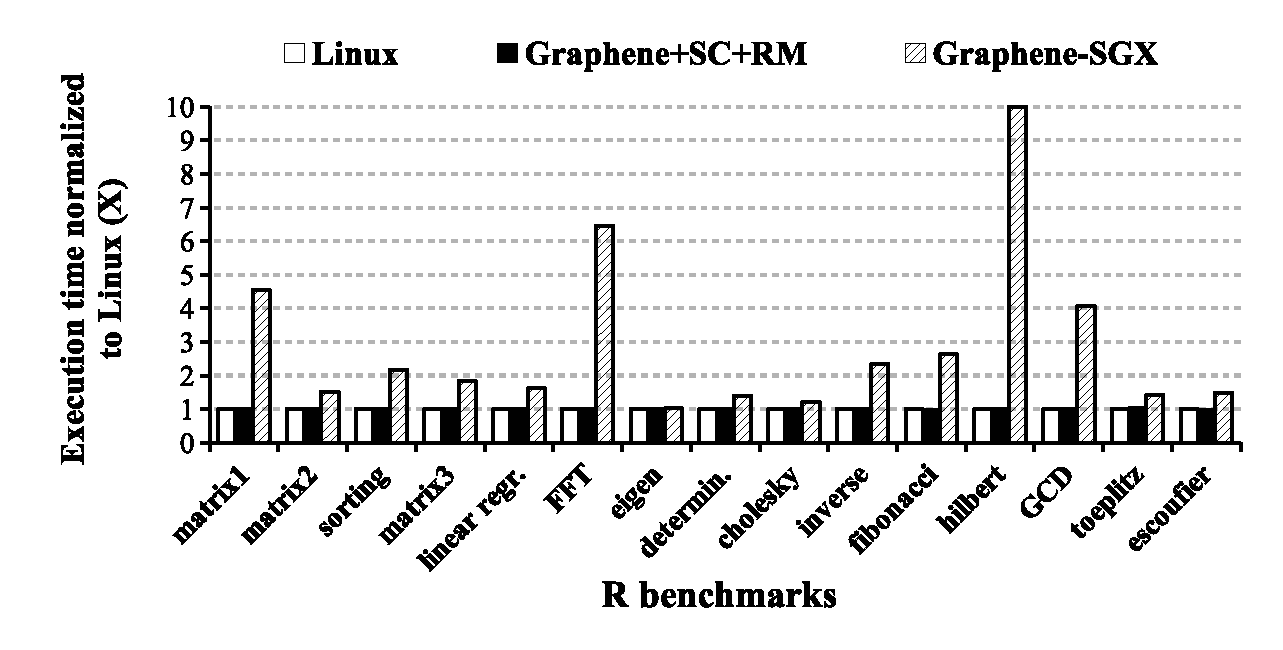
\includegraphics[width=\linewidth]{sgx/r-overhead}\\
{\bf (a) R}
\end{minipage}
\begin{minipage}{.275\textwidth}
\centering
\includegraphics[width=\linewidth]{sgx/gcc-overhead}\\
{\bf (b) GCC}
\end{minipage}
\begin{minipage}{.25\textwidth}
\centering
\includegraphics[width=\linewidth]{sgx/curl-overhead}\\
{\bf (c) CURL}
\end{minipage}

\caption{Performance overhead on desktop applications, including latency of R, execution time of GCC compilation, download time with CURL. The evaluation compares native Linux, \graphene{}, and \graphenesgx{}.} %{\bf Enclave creation time is deducted from the GCC execution time.}}
\label{fig:desktop-overhead}
\end{figure*}



\subsection{Command-Line applications}


We also evaluate the performance of a few commonly-used command-line applications.
%, to evaluate the performance of \graphenesgx{} on PCs instead of servers and clouds.
Three off-the-shelf applications are tested in our experiments:
{\bf R} (v3.2.3) for statistical computing~\cite{r-project}; {\bf GCC} (v5.4), the general GNU C compiler~\cite{gcc}; {\bf CURL} (v7.74), the default command-line web client on UNIX~\cite{curl}.
These applications are chosen because they are frequently used by Linux users,
and each of them potentially  be used 
in an enclave to handle sensitive data---either on a server or a client
machine.
% can realize profitable scenarios of using enclaves on desktop machines.



We evaluate the latency or execution time of these applications. 
%, because desktop users tend to care more about responsiveness than throughput.
In our experiments, both R and CURL have internal timing features to measure the wall time
of individual operations or executions.
%However, for other applications like GCC which does not include internal timing, evaluating the execution time can be influenced by many factors.
On a Linux host, the time to start a library OS is higher than a simple 
process, but significantly lower than booting a guest OS in a VM or
starting a container. 
Prior work measured Graphene (non-SGX) start time at 641 $\mu$s~\cite{tsai14graphene}, whereas starting an empty Linux VM takes 10.3s and starting a Linux (LXC) container takes 200 ms~\cite{agarwal15container}. 
%% dp; Note that this is MILLI seconds, not micro seconds.
%average memory footprint of an empty Linux VM, with memory deduplication, is about 96MB, . 


On SGX, the enclave creation time is relatively higher, \fixme{added more detailed number} ranging from 0.5s (a 256MB enclave) to 5s (a 2G enclave), which is a fixed cost that any application framework
will have to pay to run on SGX.
%For library OSes, the time for creating and initializing an enclave is not trivial, because it is similar to booting an lightweight OS.
% a significant part of the start-up time
% of an application is more significant, because creating enclaves is expensive.
%We consider the enclave creation time as a fixed cost for any application running in \graphenesgx{},
%and acceptable to users as long as it is responsive.
Enclave creation time is determined by the latency of the hardware and the Intel kernel driver, and is primarily a function of the size of 
the enclave, which is specified at creation time because it affects the enclave signature. %\fixmedp{although can't it grow with eadd?}.  
For non-server workloads that create multiple processes during execution,
such as GCC in Figure~\ref{fig:desktop-overhead},
the enclave creation contributes a significant portion to the execution time overheads, illustrated as a stacked bar.
%Since the enclave creation time is related to the enclave size, and unrelated to the workload,
%we deduct the enclave creation time from the execution time of GCC in Figure~\ref{fig:desktop-overhead}. \fixmedp{I think it might be better to show this as a stacked bar instead of just removing it.  Opaquely subtracting this cost doesn't seem right.  Let's discuss dp: I thought we agreed to change this...}

{\bf R}~\cite{r-project} is a scripting language often used for
data processing and statistical computation.
With enclaves, users can process sensitive data on an
OS they don't trust.
We use an R benchmark suite developed by Urbanek et al.~\cite{r-benchmark-25}, which includes 15 CPU-bound workloads such as matrix computation and number processing.
\graphenesgx{} slows down by less than 100\% on the majority of the workloads, excepts the ones which involve allocation and garbage collection: ({\tt matrix1} creates and destroys matrices, and both {\tt FFT} and {\tt hilbert} involve heavy garbage collection.)
Aside from garbage collection, these R benchmarks do not frequently interact with the host.
We further note that non-SGX \graphene{} is as efficient as Linux on all workloads, 
and these overheads appear to be SGX-specific.
%\fixmedp{Check this pontification}
In our experience, garbage collection and memory management code in managed language runtime
systems tends to be written with assumptions that do not match enclaves,
such as a large, sparse address space or that memory can be demand paged 
nearly for free (SGX version 1 requires all memory to be mapped
at creation); a useful area for future work would be to design
garbage collection strategies that are optimized for enclaves.
%we believe the overheads on \graphenesgx{} are contributed by enclaves.
 
{\bf GCC}~\cite{gcc} is a widely-used C compiler.
By supporting GCC in enclaves, developers can compile closed-source applications on customers' machines,
without leaking the source code.
GCC composes of multiple binaries, including {\tt cc1} (compiler), {\tt as} (assembler), and {\tt ld} (linker).
Therefore, GCC is a multi-process program using \syscall{execve}.
We test the compilation of thee source files with varied sizes,
using single C source files collected by MIT~\cite{gcc-benchmark}.
Each GCC execution typically \fixme{it's five, not four} creates five processes, and we run each process in a 256MB enclave by default.
%and has a fixed cost on enclave creation, which is unrelated to workload and depends on the enclave size.
%\fixme{check this}
\fixme{clarified this part, to prevent confusion between latency and overhead. also, GCC numbers got better.}
For a small workload like compiling {\tt gzip.c} (5 kLoC), running in \graphenesgx{} (4.1s) is 18.7$\times$ slower than Linux (0.2s).
The bulk of this time is spent in enclave creation, taking 3.0s in total, while the whole execution inside the enclaves, including initialization of the library OS and OS shield, takes only 1.1s, or 4.2$\times$ overhead.
For larger workloads like {\tt oggenc.c} (50 kLoC) and {\tt gcc.c} (500 kLoC), 
the overhead of \graphenesgx{} is less significant. % (3.6$\times$ and 2.1$\times$ overhead, respectively).
For {\tt gcc.c} (500 kLoC), we have to enlarge one of the enclaves ({\tt cc1}) to 2GB,
but running on \graphenesgx{} (53.1s) is only 2.1$\times$ slower than Linux (17.2s),
and 7.1s is spent on enclave creation.
%and the creation of four enclaves takes 8s.
%Each compilation has a fixed enclave creation time in \graphenesgx{}, which is about 1--2 seconds per enclave. We deduct the creation time of all enclaves  to gain more meaningful results, but do not hide rest of the overhead on fork.
%\fixmedp{Also not comfortable with this; add a bar?}
%In general, GCC in \graphenesgx{} is 1--5$\times$ slower than GCC on native Linux. 
%\fixmedp{This really needs some profiling if possible}
The overhead of non-SGX \graphene{} on GCC is marginal.
 



{\bf CURL}~\cite{curl} is a command-line  web downloader.
\graphenesgx{} can make CURL into a secure downloader that attests both server and client ends.
We evaluate the total time to download a large file, ranging from 1MB to 1GB, from another machine running Apache. % over Gigabit LAN.
%across high-speed university network\fixmedp{more specific, as above}.
\graphene{} has marginal overhead on CURL, and
\graphenesgx{} adds 7--61\% overhead to the downloading time of CURL, due to the latency of I/O.


\begin{figure*}[t!]
\centering

\begin{minipage}{.3\textwidth}
\centering
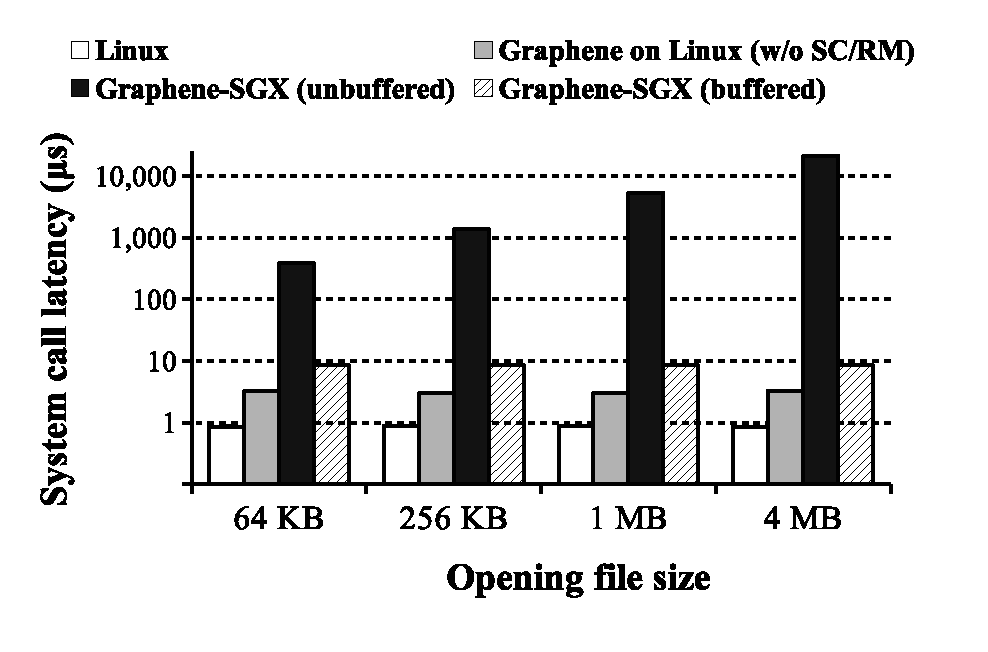
\includegraphics[width=\linewidth]{sgx/open-latency}\\
{\bf (a) Open a file}
\end{minipage}
\begin{minipage}{.3\textwidth}
\centering
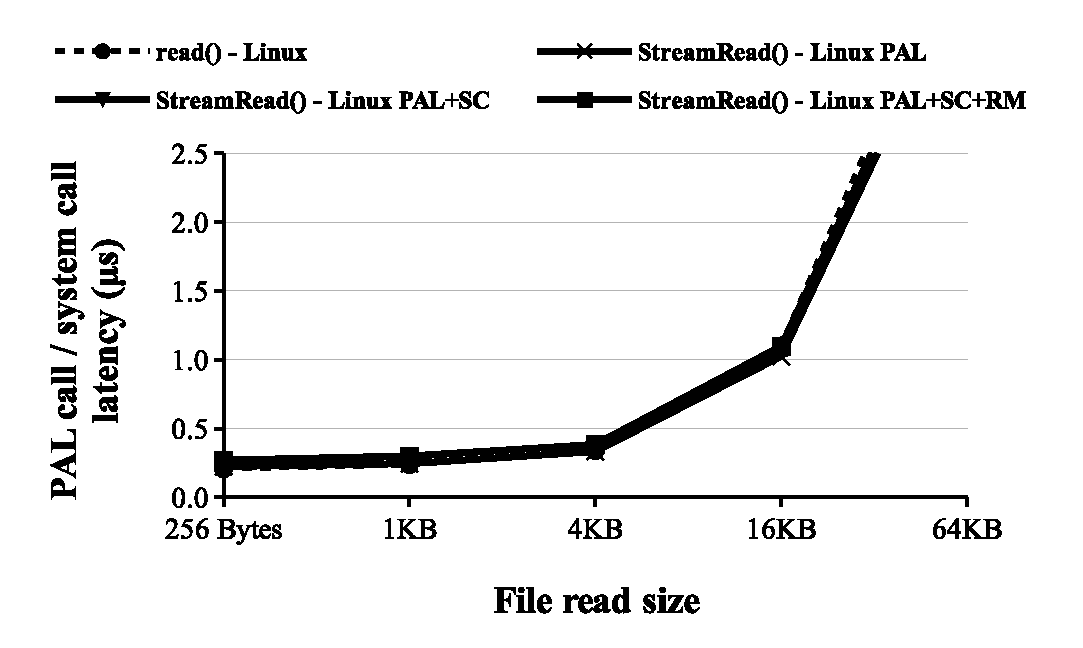
\includegraphics[width=\linewidth]{sgx/read-latency}\\
{\bf (b) Read a file}
\end{minipage}
\begin{minipage}{.3\textwidth}
\centering
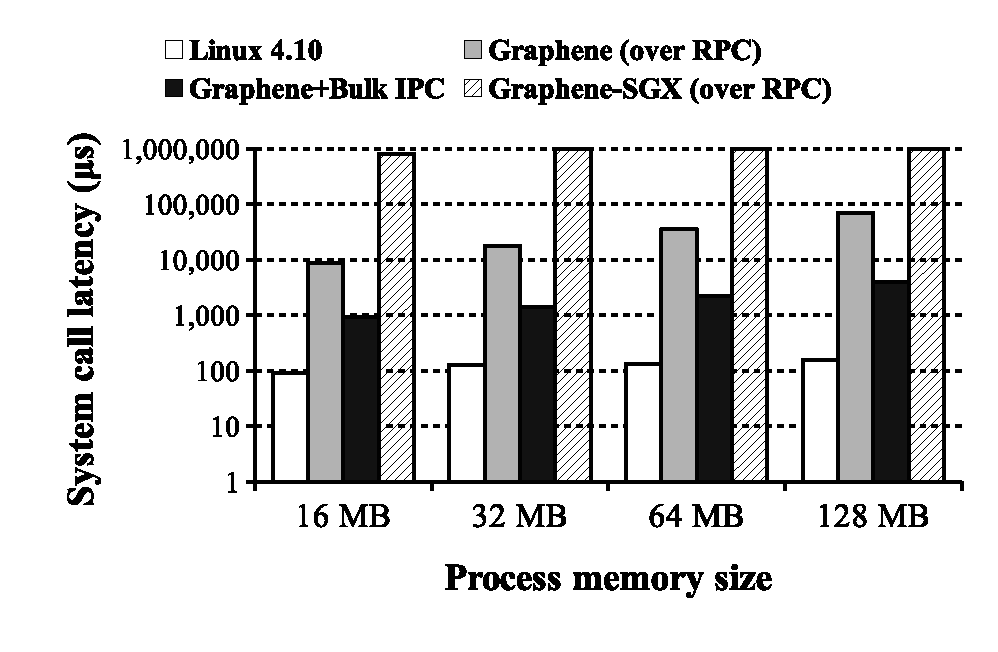
\includegraphics[width=\linewidth]{sgx/fork-latency}\\
{\bf (c) Fork a process}
\end{minipage}

\caption{Latency of some expensive system calls in \graphenesgx{}, including opening and reading a secured (authenticated) file, and forking a new process. The results are compared with native Linux and \graphene{}.}
\label{fig:syscall}
\end{figure*}


\subsection{Performance Overhead Analysis}


In this section we evaluate a few system operations that are heavily impacted by the \graphenesgx{} design.
%To shield dynamic loading and process creation,
%\graphenesgx{} uses computationally-expensive cryptographic techniques \fixmedp{more specific?} to verify enclave inputs.
% under the circumstance that the host OS cannot be trusted.
%As a trade-off to the security, the performance will be affected
%by additional cryptographic computation.
We measure the \syscall{open}, \syscall{read}, and \syscall{fork} system calls
using LMbench 2.5~\cite{McVoy:lmbench}.
A primary source of the overheads on these system calls is the cost of shielding applications, with run-time checks on the inputs.
Cryptographic techniques are used to: (1) validate the file against the secure hash, at \syscall{open}, (2) check the file chunks against the Merkle tree, at \syscall{read}, and (3) establish a TLS connection over inter-enclave RPC, at \syscall{fork}.
%opening a integrity-sensitive file for the first time, 
% or using cryptographic techniques, such as secure hashing, to verify the inputs.
% microbenchmarking specific system calls: 
% system calls,
%with different application settings.
%The microbenchmark is part of the LMBench 2.5 test suite
%\fixmedp{maybe merge this in the above paragraph, which feels a little coy}
%For instance, in order to shield dynamic loading, \graphenesgx{} checks each binary file against the secure hashes in the manifest,
%when the file is opened for the first time---after the whole file is copied into the enclave.
%\fixmedp{This happens after they are copied into enclave, memory right?}
%The verification happens when opening the file for the first time (often by the 
%After \graphenesgx{} validates the file, we generate a series of hashes of the file in chunks, as a merkle tree.
%to prevent verifying the whole file again when later randomly reading a part of the file.
%\fixmedp{So is this for the case when a file is swapped out?  I'm confused here - some details are missing}
%The latency of opening and reading an authenticated file in \graphenesgx{} is dominated by SHA256 and SHA512 calculation.
The remaining overheads contribute to exiting the enclave for host system calls, and bringing memory into the EPC (enclave page cache) or decrypting 
memory on a last-level cache miss. %and later the cache where the memory is decrypted by the CPU.


Figure~\ref{fig:syscall}(a)
shows the overhead for authenticating files in \syscall{open}.
\fixme{change overhead to latency}
Depending on the file size, the latency of \syscall{open} on \graphenesgx{} is 383$\mu$s (64KB file) to 21ms (4MB file), whereas on Linux, the latency is constant at 0.85$\mu$s.
We note that this is where enclaves are at a disadvantage, as \syscall{open} 
normally does not need to read file content; whereas here \graphenesgx{} uses \syscall{open}
as a point at which to validate file content.
For a subsequent \syscall{open}, when the Merkle tree is already generated, the overhead of simply exiting enclave for \syscall{open}, and searching the file list in the manifest, is about 9$\times$.
%\fixmedp{why?}


One might be able to optimize further for cases where only part of a file is accessed
with incremental hashing.  However, in the common case where nearly all of the file is accessed,
these costs are difficult to avoid when host file system is untrusted.
Another opportunity 
is to create the Merkle tree offline, when the manifest is created.
%\fixmedp{I think the second idea has legs...}


%This is an inevitable cost, because normal \funcname{open} on trusted OSes
%need not to access file content.
%After verifying the file, \graphenesgx{} buffers the chunk hash values, to skip whole-file verification when the file is reopened.

Figure~\ref{fig:syscall}(b)
shows the overhead for authenticating files in \syscall{read}, which 
is lower than \syscall{open}.
Since the whole file has been verified at \syscall{open}, the sequential \syscall{read} only verifies the chunks of files it is reading from untrusted memory.
%Reads from data cached in enclave memory are cheaper.  %\fixmedp{right? can we say how much cheaper?  Maybe add separate bars for both cases?}
% Therefore, \syscall{read} is actually much cheaper than \syscall{open}.
Depending on the size of blocks being read, the latency on \graphenesgx{} is 0.5$\mu$s (64-byte \syscall{read}) to 16.9$\mu$s (4KB \syscall{read}). The latency of \syscall{read} on Linux is \roughly{}0.1$\mu$s for any block size below 4KB.
If the file is not authenticated,
\graphenesgx{} only copies the file contents into the buffer, and the overhead reduces to 48\% (64-byte \syscall{read}) to 83\% (4KB \syscall{read}).
\fixmedp{Consider doing larger buffers, say up to 64k or even 4 MB}

%\fixmedp{In the legend for 7b, unsecure should be insecure}


Figure~\ref{fig:syscall}(c) shows the overhead of forking a process.
As described in \ref{sec:multiproc}, the latency of \syscall{fork} in \graphenesgx{} is affected by three factors:
creation of a new enclave, local attestation of the integrity, and duplicating the process state over an encrypted RPC stream.
Combining these factors, \syscall{fork} is one of the most expensive calls in \graphenesgx{}.
%, but at least it is supported natively on the current hardware.
The default enclave size is 256MB.
%which takes \roughly{}0.5s to create. 
Our evaluation shows that the latency of forking a process is around 0.8s (16MB process) to 2.7s (128MB process), but can be more expensive if the parent process uses more memory.
The trend matches the performance of \graphene{} without the bulk IPC optimization.
\fixmedp{If you want, some thoughts on how this might be improved in the future would be nice...  One good suggestion is recycling enclaves, or pre-forking so measurements can be done in parallel}
%Due to the overhead on \funcname{fork}, \graphenesgx{} is not suitable for fork-intensive workloads like Bash scripts
%if performance is critical.

\fixme{talk about a limitation of improving fork. check this.}
One way to further optimize \syscall{fork} is to reduce or avoid enclave creation time; one can potentially pre-launch a child enclave, and then migrate the process contents later when \syscall{fork} is called.
There might be another opportunity to improve the latency of process migration,
if copy-on-write sharing of enclave pages can be supported in future generations of SGX.
%Unfortunately, sending the process contents is difficult to avoid in \syscall{fork},
%as SGX disallows sharing enclave memory between multiple enclaves.

%\fixmedp{I assume 5.4 isn't done yet}



\subsection{TCB Size and Shielded Functionality}

In this section we measure the increase in TCB size of \graphenesgx{},
%in lines of code, 
as well as 
%compare the TCB size increased by \graphenesgx{} to an unmodified application, in lines of code, and 
the OS functionality shielded by the framework.
We compare to \scone{} and \panoply{}, using
%For SCONE and Panoply, we use 
numbers reported in their papers. 
%The conventional One generally assumes 
A smaller TCB is generally easier to review or possibly verify,
and is assumed to have fewer vulnerabilities.
%more implies lower burden for code review or formal verification, and less risk of writing exploitable code.
%For instance, Panoply argues that, because its use cases are typically smaller than 20kLoC, including both the application logic and Panoply itself, it is within the realm of future, automated verification~\cite{shinde17panoply}.

\fixmedp{Reviewer B asks for memory footprint, which isn't a bad idea}

\begin{table}
\footnotesize
\centering
\bgroup
\def\arraystretch{1.2}
\setlength{\tabcolsep}{0.5em}
\begin{tabular}{>{\raggedright\arraybackslash}p{9em}>{\raggedleft\arraybackslash\bf}p{7em}>{\raggedleft\arraybackslash}p{4.25em}>{\raggedleft\arraybackslash}p{4.25em}}
Components                    & \graphenesgx{}  & \scone{}     & \panoply{}  \\
\hline
libc (ld, libm, pthread)      &  1,292 &   88 & --      \\
                              & (glibc-2.19) & (musl)   &          \\
Library OS                    &     34 &  --      & --     \\
PAL / OS Shield               &     22 &   99 & 10  \\
\hline
Total                         &  1,348 &  187 & 10  \\
\hline
\end{tabular}
\egroup
\caption{TCB size (in thousands of lines of code) of \graphenesgx{}, \scone{}, and \panoply{}.}
\label{tab:tcb-size}
\end{table}

Table~\ref{tab:tcb-size} lists the lines of code in each components within the TCB of \graphenesgx{}, \scone{}, and \panoply{}.
By comparing the total TCB size, \graphenesgx{} is 9$\times{}$ larger than \scone{}, and 134$\times{}$ larger than \panoply{}.
However, the primary difference is the selection of libc: 
for maximum compatibility, \graphene{} uses glibc.
\scone{} uses the smaller musl libc, which lacks some features of glibc.
%it would be easy to use the smaller, and incomplete, musl libc.
%SCONE uses 
% Linux applications, \graphenesgx{} chooses to use a minimally-modified glibc, whereas SCONE uses the much more lightweight musl and 
\panoply{} excludes libc from its TCB,
% \fixmedp{what is their rationale, again? Check this}
to fit into the range of automated formal verification,
as they shield at the libc interface.
In principle, \graphene{} could easily support musl as well as glibc for applications
that do not need the additional features of glibc.
We also see the benefit of removing unused code from 
libraries, especially in an unsafe language,
similar to the approach taken in unikernels~\cite{unikernels}.
On balance, 
this choice of libc implementation is largely orthogonal to the issue
of how general-purpose the shields are.

%We argue that the choice of libc is orthogonal to the design of \graphenesgx{}; one can statically compile the applications against musl or glibc if TCB size is a concern, or given plenty of time, trim the libc functionality to bare minimum. 

If we focus on the TCB size of the library OS and the shields, 
\graphenesgx{} is 
%library OS and PAL in \graphenesgx{}, with the shielding layer of SCONE, we are 
44\% smaller than \scone{}. 
We cannot analyze the size of \scone{} because it is closed source.
%, although
%we suspect
%Although it is unclear what is in the implementation of SCONE, because it is not yet open-sourced, we believe the largest portion of their TCB contributes to the cryptography library.
\panoply{} has a smaller TCB in its shield, but within the same order of magnitude.
Panoply only shields 91 out of 256 supported POSIX functions; for context, POSIX 1003.1 defines 1,191 APIs~\cite{POSIX1003-1-2008}.
%out of 256 currently supported by \panoply{} \fixmedp{The better number is how many total functions in POSIX}.

All three of these compatibility layers or shields are within the same
order of magnitude in code size, and the differences are likely 
correlated with different ranges of supported functionality.
A recent study indicates that only order-of-magnitude differences in code
size correlate with reported CVE vulnerabilities; within the same order-of-magnitude,
the data is inconclusive that there is a meaningful difference in risk~\cite{security-metric}.
Thus, increased generality does not necessarily come with 
increased risk. % is not a clear relationship between risk 

% data only correlates
%with differences in code size when 

%Besides the choice of libc, we argue that the TCB size of a library OS or a shim shielding layer is actually correlated with the functionality that it supports or shields. Because none of the three frameworks have completely shielded the whole Linux system call table or POSIX, it is unclear how much code has to be added in the future. \graphenesgx{} also shows that one can always engineer a library OS with a small TCB, if most code is not reused from a monolithic OS kernel like Windows or Linux.
%A recent study of the CVE database also points out that having a larger TCB does not necessarily indicate more vulnerabilities, even when the difference is more than two order-of-magnitude. 



\input{apistudy}

\makeatletter
\def\input@path{{}}
\makeatother
\graphicspath{{}}
\section{Conclusion}

This paper demonstrates that the costs of running an unmodified application in SGX on a library OS are
marginal compared to thinner shims.
The major costs of using SGX are still hardware limitations of SGX.
As SGX and similar technologies mature, these design choices may have more impact.
In the interim, \sysname{} serves as a simple, open-source tool to quickly bring up
existing applications on SGX, and then incrementally adapt the code to improve performance and security on SGX.
%\fixme{Mona suggests dropping this}
%We believe the \sysname{} design is sufficiently general that porting applications to AMD's PSP
%features should only require porting the PAL.
%\fixme{Mona suggest adding this argument:
%``Graphene-SGX can provide support for running unmodified applications on SGX that provide encryption and integrity Vs SEV that can run unmodified applications, but provides only encryption but no integrity guarantees.''}

\section*{Acknowledgements}

We thank the anonymous reviewers, Vyas Sekar, and our shepherd, Bryan Ford,
for insightful comments on earlier drafts of this paper.
Anchal Agarwal, Amit Arya, Imran Brown, Gurpreet Chadha, Naveen Kalaskar, Manikantan Subramanian, and Sourabh Yerfule contributed to the \sysname{} prototype implementation.
\fixmedp{Make sure we didn't miss anyone.  Old authors, thomas, ...}


%\input{acknowledgements}
\bibliographystyle{abbrv}
\balance
\bibliography{../bibliography}

%\theendnotes
\end{document}
